\documentclass[11pt]{cernrep}
\usepackage{graphicx,epsfig}
\bibliographystyle{lesHouches}

\usepackage{cite}
\usepackage{amsmath}
\usepackage[colorlinks=True,citecolor=blue]{hyperref}
\usepackage{lscape}
\usepackage{amsmath,amssymb}

\usepackage{subfigure}

\newcommand{\GeV}{\,\mathrm{GeV}}
\newcommand{\TeV}{\,\mathrm{TeV}}
\newcommand{\ie}{i.e.\ }
\newcommand{\eg}{e.g.\ }
\newcommand{\order}[1]{{\cal O}\left(#1\right)}
\newcommand{\avg}[1]{\left\langle\smash{#1}\right\rangle}
\newcommand{\as}{\alpha_s}
\newcommand{\ycut}{y_{\text{cut}}}
\newcommand{\zcut}{z_{\text{cut}}}
\newcommand{\fcut}{f_{\text{cut}}}
\newcommand{\ftrim}{f_{\text{trim}}}
\newcommand{\Rtrim}{R_{\text{trim}}}
\newcommand{\rtrim}{r_{\text{trim}}}
\newcommand{\zprune}{z_{\text{prune}}}
\newcommand{\Rprune}{R_{\text{prune}}}
\newcommand{\rprune}{r_{\text{prune}}}
\newcommand{\e}{\varepsilon}
\newcommand{\cf}{C_{F}}
\newcommand{\ca}{C_{A}}
\newcommand{\nf}{n_{F}}
\newcommand{\MSb}{\overline{\rm MS}}
\newcommand{\W}{{\rm W}}
\newcommand{\TiTj}{{\bf T}_i \cdot {\bf T}_j}
\newcommand{\ord}{\mathcal{O}}
\newcommand{\gstrong}{g_s}
\newcommand{\muNP}{\mu_\text{NP}}
\newcommand{\amax}{a_2}
\newcommand{\amin}{a_1}
\newcommand{\tlambda}{\tilde{\lambda}}



\renewcommand{\d}{\mathrm{d}}

\newcommand{\SD}{SoftDrop\xspace}
\newcommand{\ttt}[1]{{\small\texttt{#1}}}
\newcommand{\fastjet}{\texttt{FastJet}\xspace}
\newcommand{\fjcontrib}{\texttt{fjcontribtJet}\xspace}

\usepackage{color}
\definecolor{darkgreen}{rgb}{0,0.5,0}
\definecolor{darkblue}{rgb}{0,0,0.7}
\definecolor{darkred}{rgb}{0.5,0,0.0}

\newcommand{\sm}[1]{\textbf{\color{darkgreen}  [#1 -- sm]}}


\begin{document}

\section{Jet Studies: Four decades of gluons\protect\footnote{Section coordinators: S.~Marzani and B.~Nachman.}$^{,}$~\protect\footnote{Contributing authors: S.~Amoroso, P.~Azzurri, H.~Brooks, S.~Forte, P.~Gras, Y.~Haddad, J.~Huston, A.~Larkoski, M.~Le Blanc, P.~Loch, K.~Long, E.~Metodiev, D.~Napoletano, S.~Prestel, P.~Richardson, F.~Ringer, J.~Roloff, D.~Soper, G.~Soyez, V.~Theeuwes.}}

Studies related to gluon jets have played a key role in particle and nuclear physics since their discovery at PETRA exactly (to the day!) \textbf{four decades} prior to the 2019 Les Houches workshop.  This section investigates gluon fragmentation at the LHC, covering nearly \textbf{four decades} in energy scales.  Low energy scales involving gluon (sub)jets are studied from the point of view of hadronization and Monte Carlo tuning.  Higher-order effects in parton shower programs are investigated using deep learning.  Gluon jet rejection is considered in the context of vector boson fusion/scattering processes.  One of the main studies at this Les Houches was a study about the usefulness of a gluon jet differential cross section measurement in the context of parton distribution functions.  Gluon jet identification was also briefly discussed for searches at the highest energies accessible at the LHC.

\subsection{Introduction}
\label{sec:jets:intro}

Jets are collimated sprays of hadrons that emerge from high energy quarks and gluons and are an important asset or significant nuisance in a a majority of collider particle physics analyses.  Understanding jets and their internal structure (jet substructure~\cite{Abdesselam:2010pt,Altheimer:2012mn,Altheimer:2013yza,Adams:2015hiv,Asquith:2018igt,Larkoski:2017jix,Marzani:2019hun}) will directly or indirectly address a variety of fundamental questions in particle and nuclear physics.  One of the first studies related to jet substructure occurred nearly four decades ago, with the direct discovery of the gluon at PETRA~\cite{Brandelik:1979bd,Barber:1979yr,Berger:1979cj,Bartel:1979ut,Ellis:2014rma}.  It was of paramount importance at the time to study differences between jets initiated by quarks (quark jets) and jets initiated by gluons (gluon jets) in order to categorize the properties of the new boson.  This complex topic is still an active area of research in the present day and was the subject of the 2015 Les Houches report on jets~\cite{Badger:2016bpw,Gras:2017jty}.   The goal of this report is to study gluon jets at all relevant energies at the LHC, from non-perturbative scales all the way to the highest accessible energies.   Traversing nearly four decades in energy scales will reveal a plethora of interesting phenomena.  

At the lowest energies, jets are dominated by non-perturbative effects.  While there has been significant progress in understanding jet formation when fixed-order or resummed perturbation theory is accurate, there has been much less progress outside these regions of phase space.  While such contributions are often small for most observables, they are relevant for any precision program involving hadronic final states.  One example is the determination of the strong coupling constant, $\alpha_s$, from hadronic event shapes~\cite{Abbate:2010xh,Hoang:2015hka,TheALEPHCollaboration2004,DELPHICollaboration1997,Abdallah:2004xe,Biebel:1999zt,Abbiendi:2004qz,Buskulic:1992hq}.   After lattice determinations, the most precise extractions of $\alpha_s$ use thrust and the $C$-parameter from $e^+e^-$ data.  One of the biggest challenges of this extraction is that the non-perturbative corrections are nearly degenerate with changes to $\alpha_s$~\cite{Abbate:2010xh}.  The 2017 Les Houches report on jets studied the possibility of using jet substructure at the LHC to determine $\alpha_s$~\cite{Bendavid:2018nar}.  A key ingredient to this study is jet grooming, which is a set of tools to systematically remove soft and wide angle radiation within a jet.  Well-designed grooming algorithms allow for precise theory predictions of certain observables in part because the magnitude and the onset of non-perturbative effects can be parametrically suppressed with respect to the un-groomed case.  While jet grooming may not be enough to eliminate the need to estimate non-perturbative effects, grooming may provide a unique opportunity to isolate these effects for further study.   While the perturbative regions of phase space have received significant attention from the community~\cite{Frye:2016aiz,Frye:2016okc,Marzani:2017mva,Marzani:2017kqd,Kang:2018vgn,Kang:2018jwa,Baron:2018nfz,Kardos:2018kth}, the non-perturbative regions have only recently been investigated~\cite{Hoang:2019ceu}.   One of the goals of this report is to explore the non-perturbative region of groomed jets using phenomenological tools for guidance. 

Both perturbative and non-perturbative regions of phase space at low energy can be important inputs to Parton Shower Monte Carlo (PSMC) parameter tuning.  In particular, there is a need for data enriched in gluon jets as many of the existing tunes are either based solely on or are anchored based on $e^+e^-$ data.  While those data are free from many nuisances like the underlying event, they are dominated by quark jets.  Various tuning campaigns at the LHC have found potential sources of tension between tunes that use jet substructure from the LHC and those that use jet and event shapes from LEP~\cite{ATL-PHYS-PUB-2014-021,Aad:2016oit}.  It is therefore critical to collect new measurements with unique and overlapping sensitivity to a variety of phase space regions.  The community repository for storing measurements is HepData~\cite{Buckley:2010jn,Maguire:2017ypu} and the standard for encoding an analysis for reinterpretation is Rivet~\cite{Buckley:2010ar}.  In the preparation of this report, new routines have been added to the existing databases and a list of jet substructure measurements from the LHC experiments has been tabulated.

While many aspects of PSMC programs are built on phenomenological models that must be tuned to data, there are also a variety of components that are based on fundamental aspects of the strong force and can be systematically improved.  Various MC programs such as \textsc{Dire}, \textsc{Vincia}, and \textsc{Deductor} include various subleading resummation, helicity, and color corrections.  In particular, the \textsc{Dire} program, which is a plugin to both \textsc{Pythia} or \textsc{Sherpa} now includes all of the next-to-leading order components of the QCD splitting functions including the triple-collinear and double-soft splittings.   The 2017 Les Houches report briefly reported an investigation of standard jet substructure observables (such as the two-prong tagger $N_2$~\cite{Moult:2016cvt}) to the triple collinear splitting function~\cite{Bendavid:2018nar}.  A non-exhaustive list of such observables showed no sensitivity to this splitting function.  In order to know if any jet observable is sensitive to the extended physics modeling, deep neural network classifiers were constructed using the full observable jet phase space (kinematics and particle types).   This study confirmed that the triple-collinear splitting function is essentially non-observable, but the neural networks were able to significantly detect the double-soft splitting function.  Future work is required to construct simple observables that may become near-future measurements for probing this in data.

Jet classification techniques have been used for a variety of other tasks, including quark versus gluon (q/g) jet tagging.  In the context of Les Houches 2019, the focus of q/g tagging was on the isolation of vector boson fusion (VBF) and vector boson scattering (VBS) processes.  These processes are distinguished in part by two moderate $p_T$ forward quark jets.  In the context of Higgs production, quark/gluon tagging is useful both for separating the Higgs from other Standard Model backgrounds as well as separating different Higgs production modes.   The usefulness of q/g tagging to distinguish the gluon fusion (ggH) and VBF Higgs production modes was first investigated by CMS~\cite{Khachatryan:2015bnx}.  This report will show additional studies to understand the interplay between q/g tagging and other analysis selections such as requiring a large dijet invariant mass ($m_{jj}$).

While q/g tagging has traditionally been used to \textit{reject quarks}, there may also be a physics case for tagging gluons.  One possibility in particular is the possibility of using gluon jets to constrain the gluon parton distribution function (PDF).  The gluon PDF has a large uncertainty at high $x$ ($m_{jj}\sim 1$ TeV) because the existing inclusive jet data are dominated by $qq$ initial states and $gg$ constraints from $t\bar{t}$ production become statistically limited.  What if one could directly measure the $gg$ reaction cross section?  The first step in answering this question is to establish a strong correlation between the initial and final state flavors.  This means that gluon tagging the final state will bias the initial state to be more gluonic.   The second step is to identify the tradeoff between tagging performance and uncertainties.  If the current PDF uncertainty can be made larger than the statistical and systematic uncertainties, new data would be useful in constraining the gluon PDF.  Lastly, it is important that the gluon tagging strategy is theoretically well-understood so that it can be simultaneously calculated with the $p_T$ spectrum as input to the PDF fits.  For this purpose, a new observable is considered - the \textit{Les Houches multiplicity} $n_\text{LH}$, first proposed in Ref.~\cite{Marzani:2019hun} as a variation on the iterative soft drop multiplicity~\cite{Frye:2017yrw}.

At the kinematic limit of LHC jets, gluon tagging may also have an important role for searches for new particles.  While not studied extensively at Les Houches, there was a general brainstorming session for gluon tagging applications and one promising example is the search for $X\rightarrow gg$.  At high $m_{jj}$, the SM background is dominated by valence quark scattering.  Furthermore, gluon tagging is more useful at high $p_T$ where counting observables like $n_{LH}$ have a better q/g tagging performance.  For these reasons, gluon tagging has an interesting potential to increase the sensitivity of the high mass dijet search.
%https://arxiv.org/pdf/1912.03511.pdf

This remainder of this chapter is organized from low to high energy3.  Section~\ref{sec:jets:np} begins with studies related to non-perturbative aspects of jets after grooming.  Then, Sec.~\ref{sec:jets:mc} investigates the potential for jet substructure observables for PSMC tuning.  Next, section~\ref{sec:jets:psmc} presents methods for probing higher-order effects in PSMCs.  A brief study of q/g tagging in the context of VBF/VBS is highlighted in Sec.~\ref{sec:jets:vbsbvf}.  At higher energies, the feasibility of Suppressing QUarks in the Region of RElatively Large-$x$ (\textsc{Squirrel}) is studied for the gluon PDF in Sec.~\ref{sec:jets:pdf}.  The kinematic limit is briefly described in Sec.~\ref{sec:jets:highest} and the chapter ends with conclusions and outlook in Sec.~\ref{sec:jets:conclusion}.

\subsection{Non-Perturbative effects at low jet mass}
\label{sec:jets:np}

Jet grooming is the systematic removal of soft and wide-angle emission from inside a jet.  Advances in jet grooming have resulted in algorithms like soft drop and the modified mass drop tagger (mMDT)~\cite{Larkoski:2014wba,Dasgupta:2013ihk} that are amenable to high order resummation.   Both ATLAS~\cite{Aaboud:2017qwh,Aad:2019vyi} and CMS~\cite{Sirunyan:2018xdh} have measured the soft drop jet mass and compared the differential cross section with theoretical calculations~\cite{Frye:2016aiz,Frye:2016okc,Marzani:2017mva,Marzani:2017kqd,Kang:2018vgn,Kang:2018jwa,Baron:2018nfz,Kardos:2018kth}.  As the level of both experimental and theoretical precision improves, it is natural to consider what are the next challenges.  The reconstruction and prediction of jet masses near the non-perturbative regime $k_T\lesssim \Lambda_\text{QCD}$ is becoming just as if not more important than improving the experimental and theoretical precision at medium and high masses.

At the same time, jet grooming also offers an exciting opportunity to study non-perturbative effects in isolation.  In particular, non-perturbative corrections to the jet mass are localized after jet grooming.  This is illustrated in Fig.~\ref{fig:jets:np:illustration}.  Turning on and off non-perturbative modeling in Pythia lead to an $\mathcal{O}(1)$ effect in the differential cross section, but only at low jet masses.  The goal of this section is to use phenomenological tools to investigate this structure in more detail.  This region of the phase space is particularly hard to measure experimentally and has thus far largely been avoided.  However, innovations in mass reconstruction will improve the precision at low mass and this region may be well-suited for non-perturbative studies including phenomenological model tuning.  Analytic approaches to also probe this region are also an important complement to these studies and have begun with the recent work in Ref.~\cite{Hoang:2019ceu}.

\begin{figure}[h!]
\centering
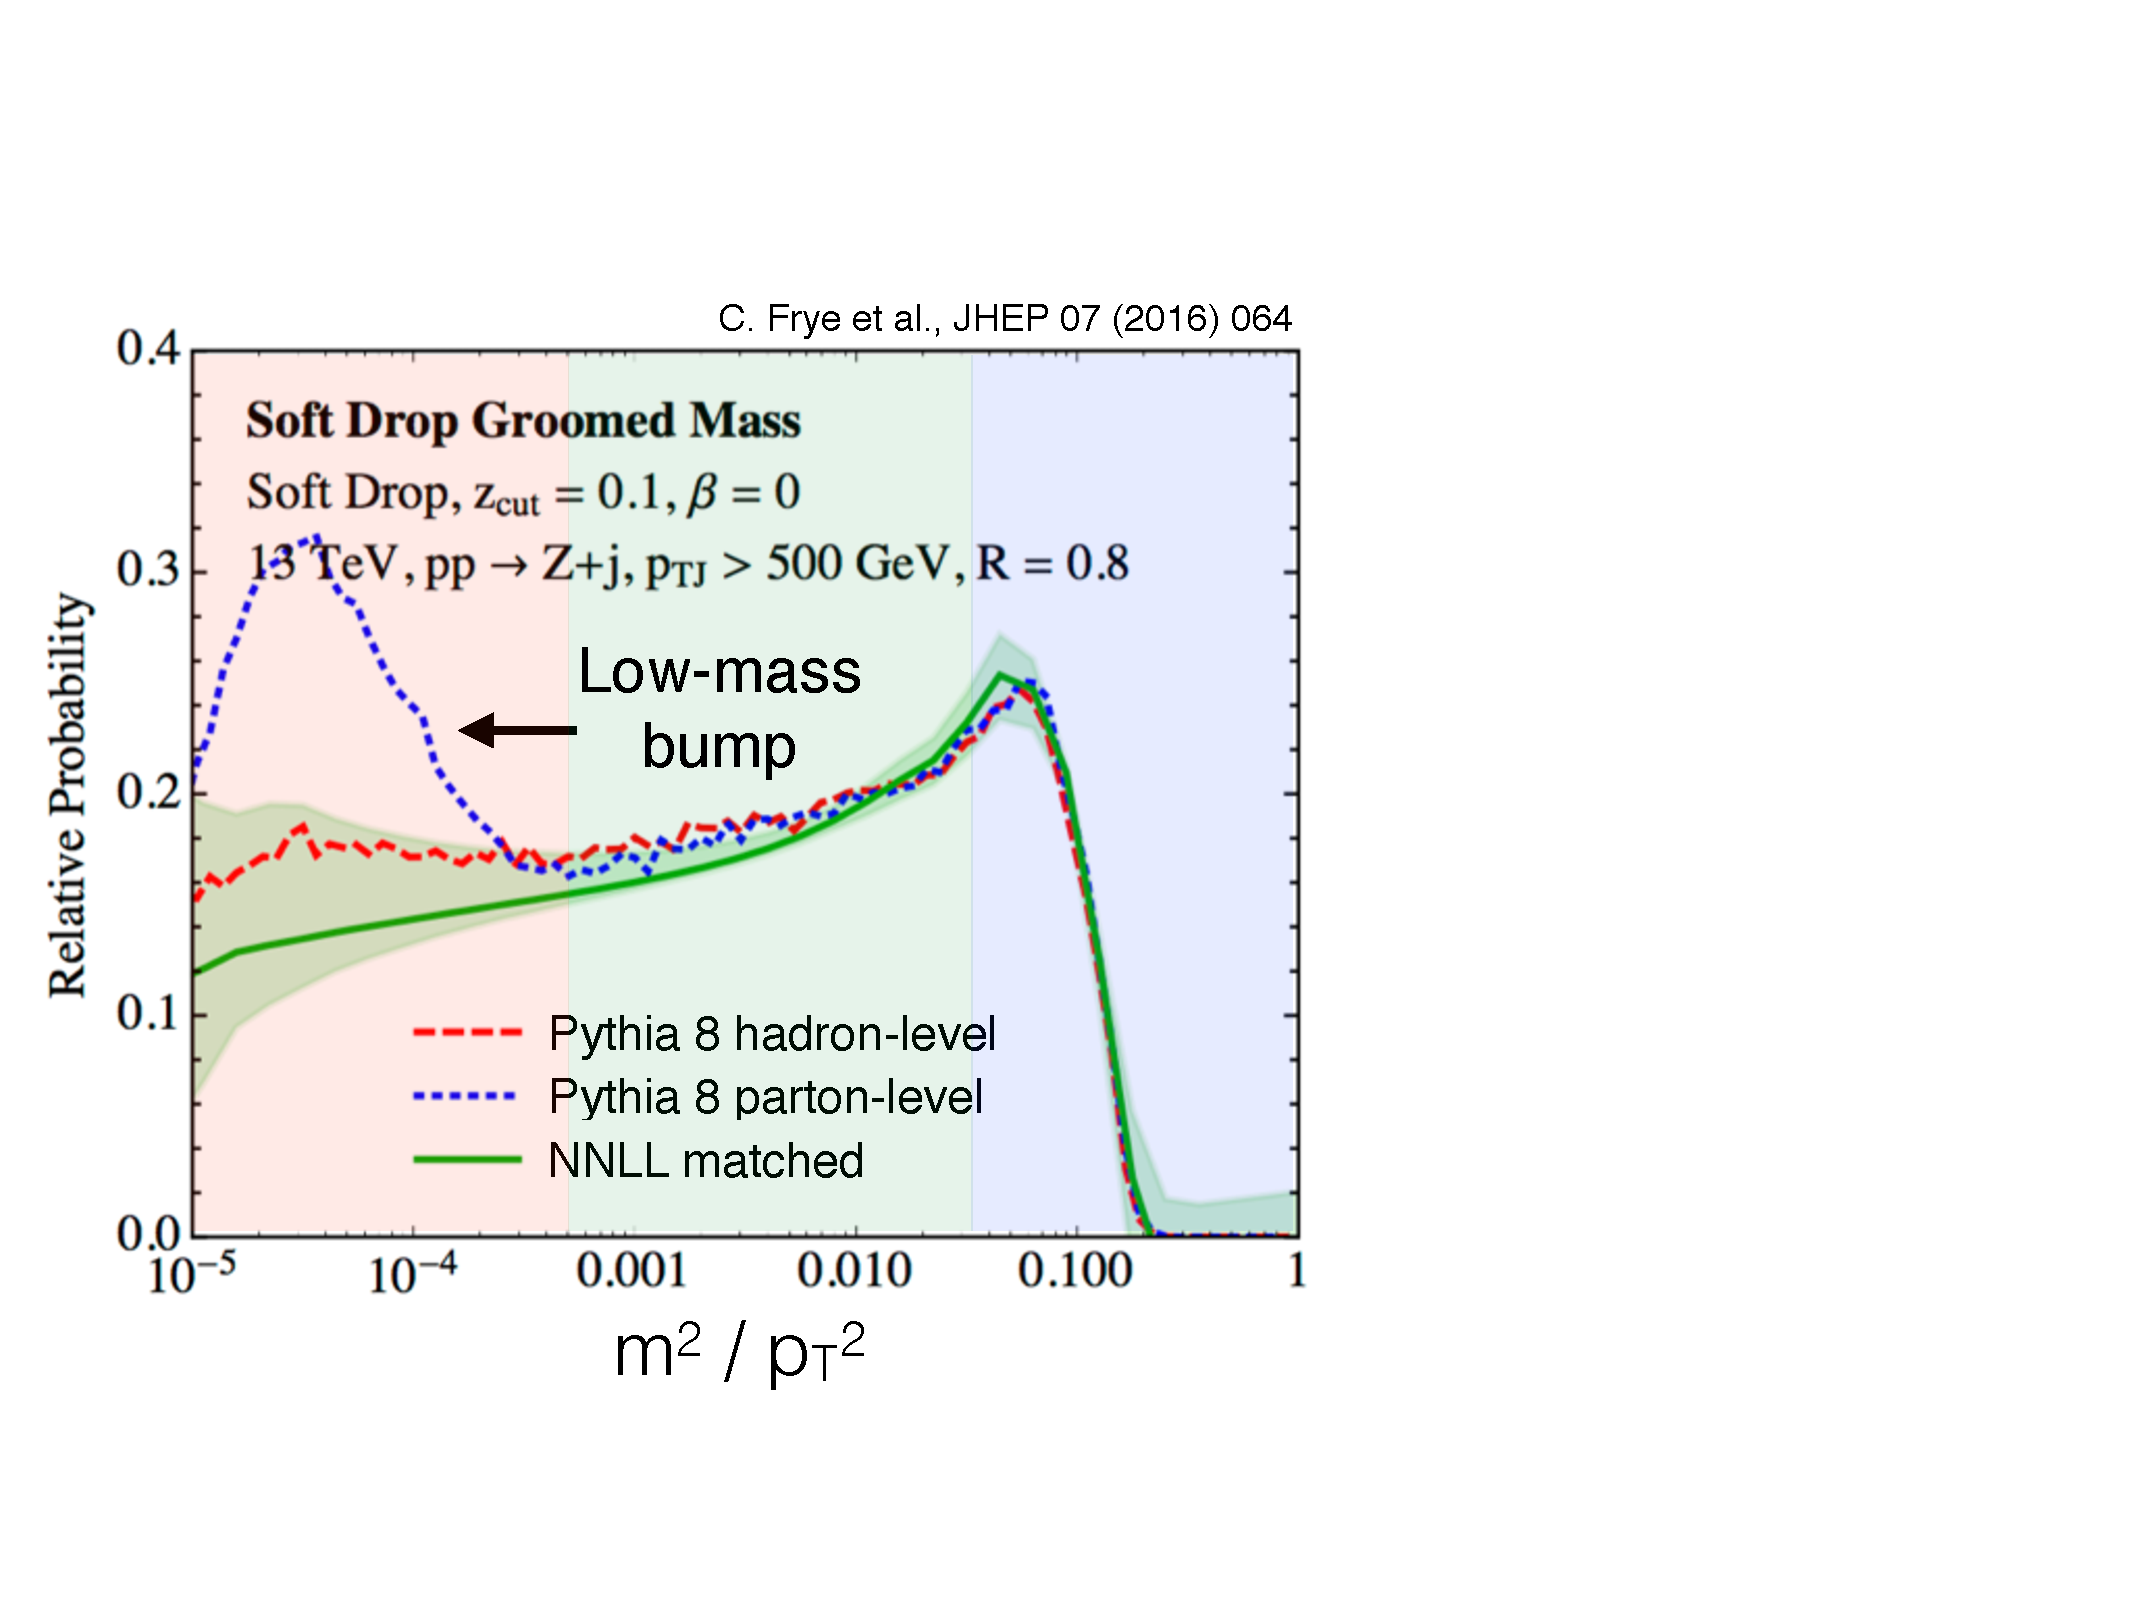
\includegraphics[width=0.6\textwidth]{figs/Lowmassbump.pdf}
\caption{Figure adapted from Ref.~\cite{Frye:2016aiz}.  The differential cross-section has three regimes: the left part (red) where non-perturbative effects dominate, the middle (green) regime where resummation is most accurate, and the right (blue) regime where fixed-order effects are the most relevant.}
\label{fig:jets:np:illustration}
\end{figure}

Figure~\ref{fig:jets:np:qg} shows the groomed jet mass predicted for dijet events using Pythia and Herwig and separated into quark jets and gluon jets.  The soft drop grooming algorithm is used with the most aggressive grooming parameter $\beta=0$ (this also corresponds to mMDT).  The leading logarithm prediction for the differential cross section in the intermediate mass region ($-3\lesssim\log_{10}(m^2/p_T^2)\lesssim -2$) is a linear distribution with the slope proportional to the QCD color factor and $\alpha_s$.  For this reason, the quark distribution is flatter with respect to the gluon distribution.  In the absence of non-perturbative effects, these trends would continue down to arbitrarily small masses. Interestingly, the non-perturbative corrections are very different for quarks and gluons, with a much larger bump for quarks.  Furthermore, the corrections for Pythia and Herwig gluons are qualitatively different, with a clear peak for Pythia gluons and the absence of a peak for Herwig.

\begin{figure}[h!]
\centering
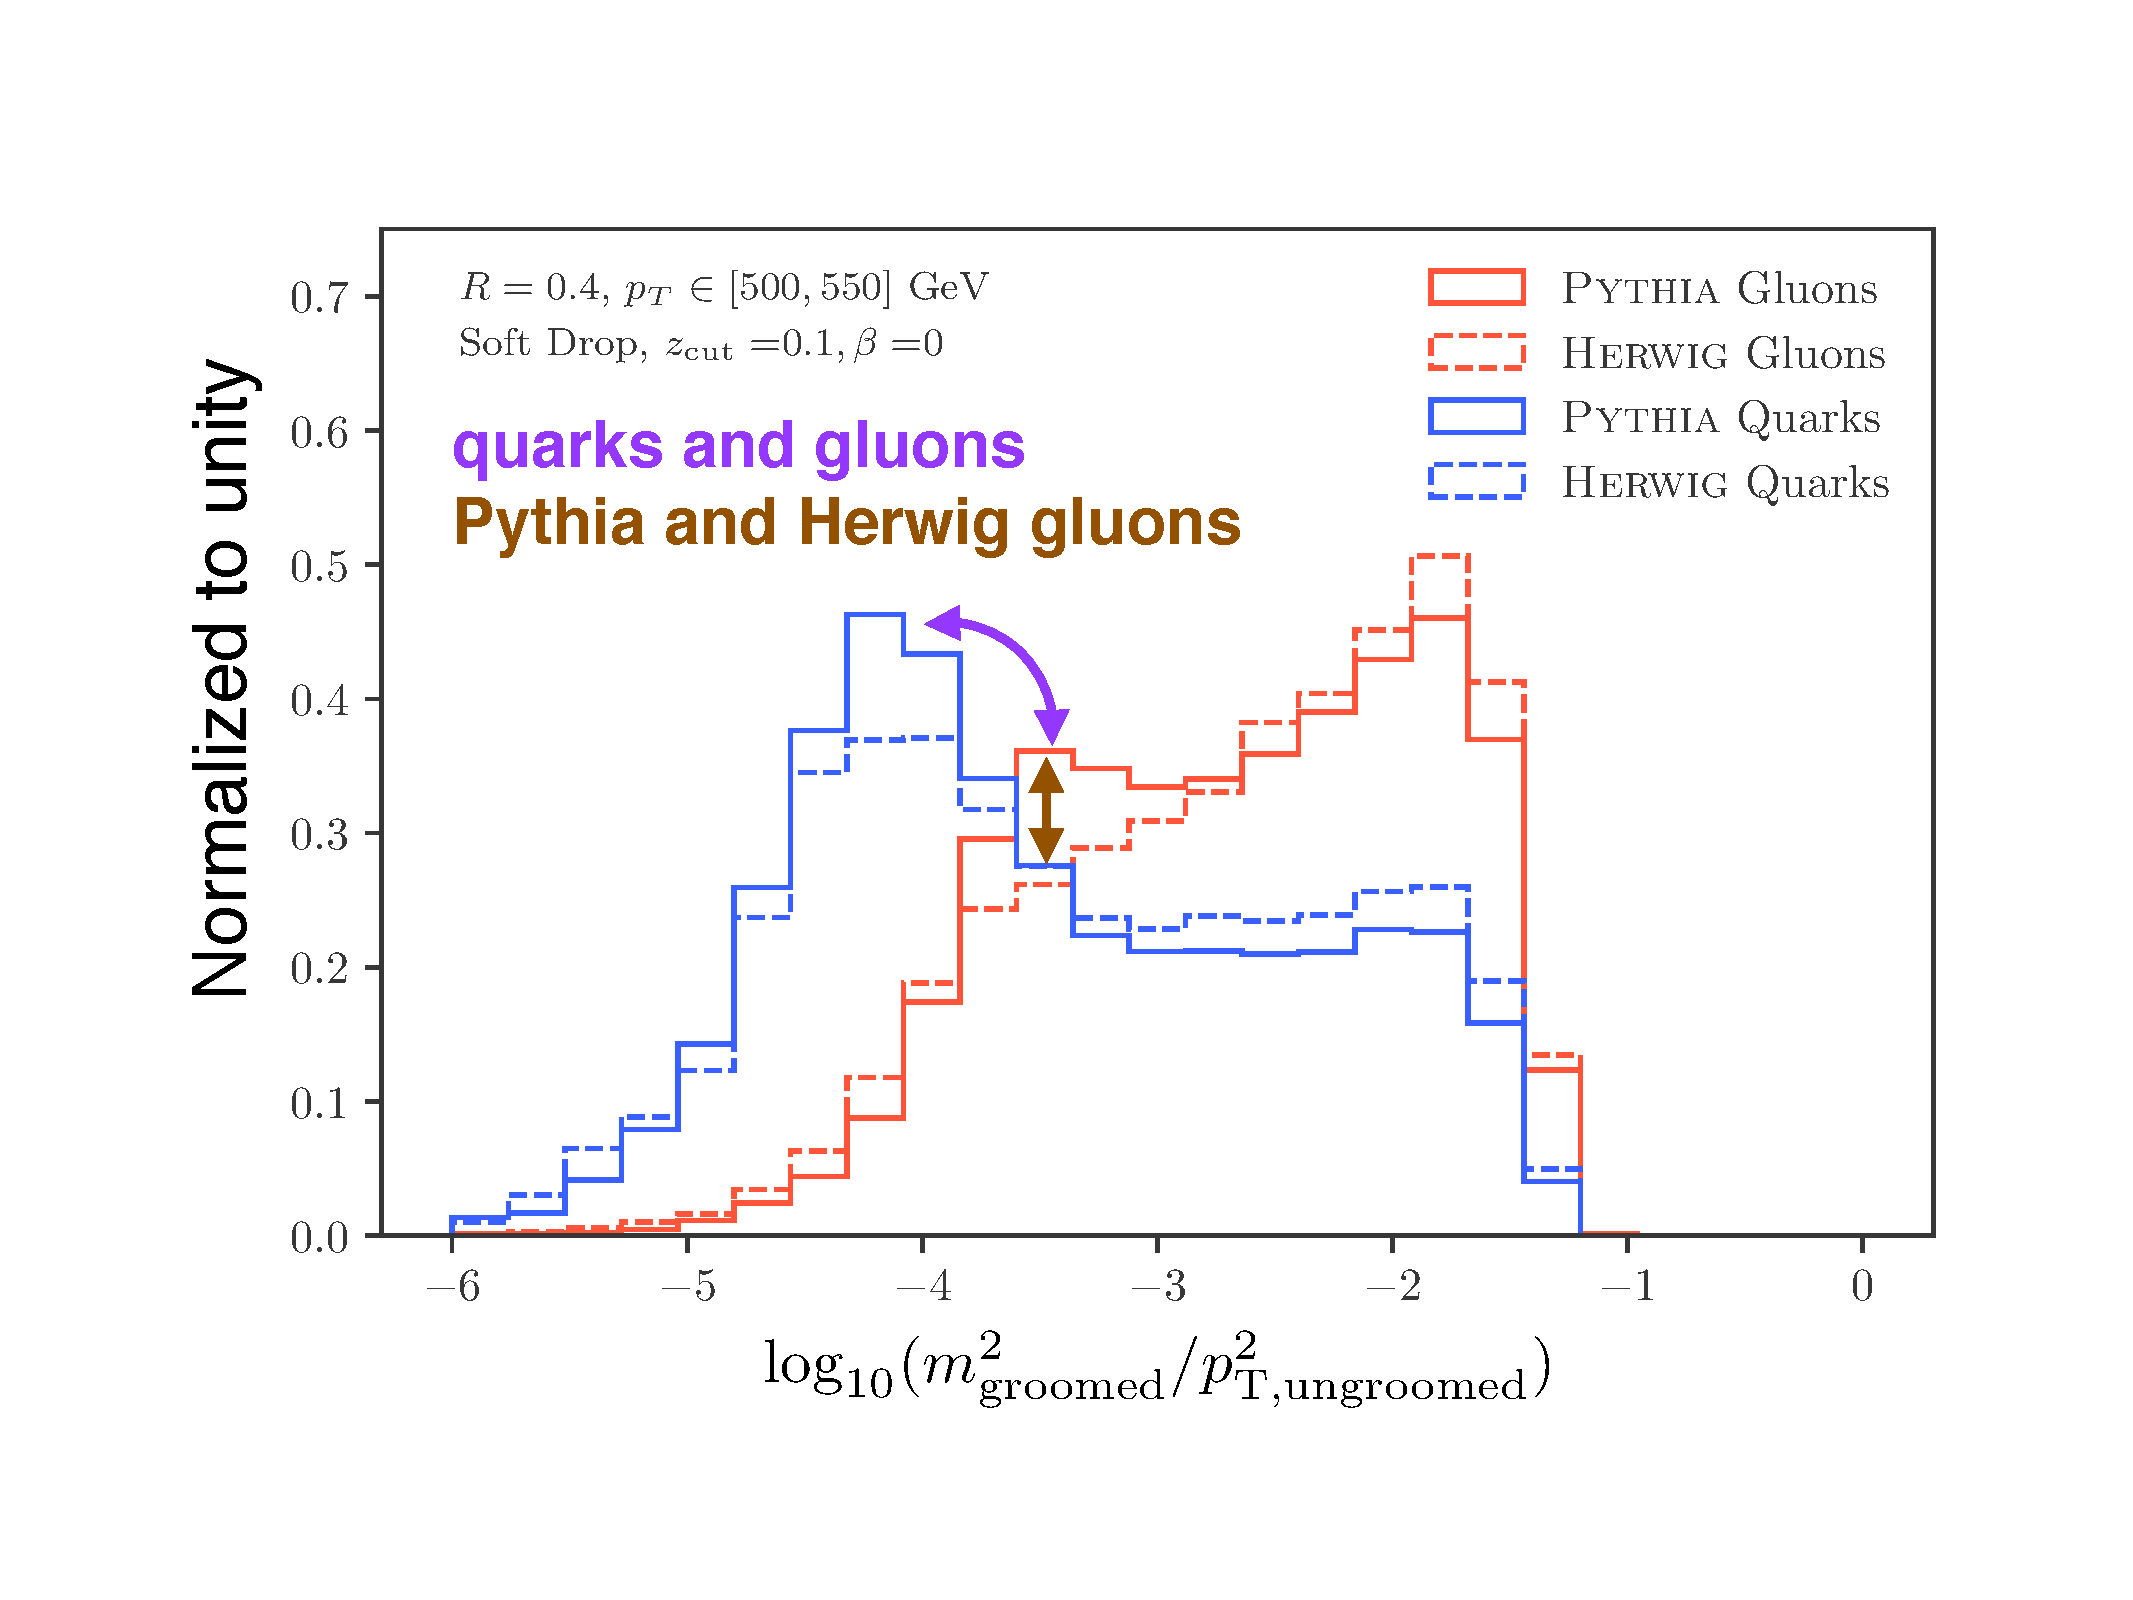
\includegraphics[width=0.6\textwidth]{figs/NPbumpvariations.pdf}
\caption{The binned differential cross-section for the groomed jet mass using Pythia and Herwig and separately for quark and gluon jets.}
\label{fig:jets:np:qg}
\end{figure}

The large model-dependence for gluon jets in Fig.~\ref{fig:jets:np:qg} motivated further studies.  It was found that the differences between quarks and gluons and between models were unrelated to gluon splitting to heavy flavor quarks and to specific hadronic resonances.  The effects are nearly 100\% correlated with jet constituent multiplicity.  Furthermore, the results depend strongly on the grooming parameters ($\beta$ and $z_\text{cut}$).  Additional studies are illustrated in Fig.~\ref{fig:jets:np:tracks}.  In particular, the blue and green lines fix everything about the simulation except for the hadronization model.  For $\lesssim\log_{10}(m^2/p_T^2)\lesssim -5$, there are $\mathcal{O}(1)$ differences between models while the rest of the spectrum is nearly unchanged, as expected.  However, this region is not probed differentially in the most recent ATLAS and CMS jet mass measurements.  The left plot of Fig.~\ref{fig:jets:np:tracks} shows that the entire region of interest for the large non-perturbative effects is covered by a single measurement bin.  The experimental jet mass resolution is poor in this region due to finite calorimeter granularity.  The right plot of Fig.~\ref{fig:jets:np:tracks} shows that the trends are largely preserved when only using tracking information, which has the potential to provide the necessary precision to probe the non-perturbative region in detail.

\begin{figure}[h!]
\centering
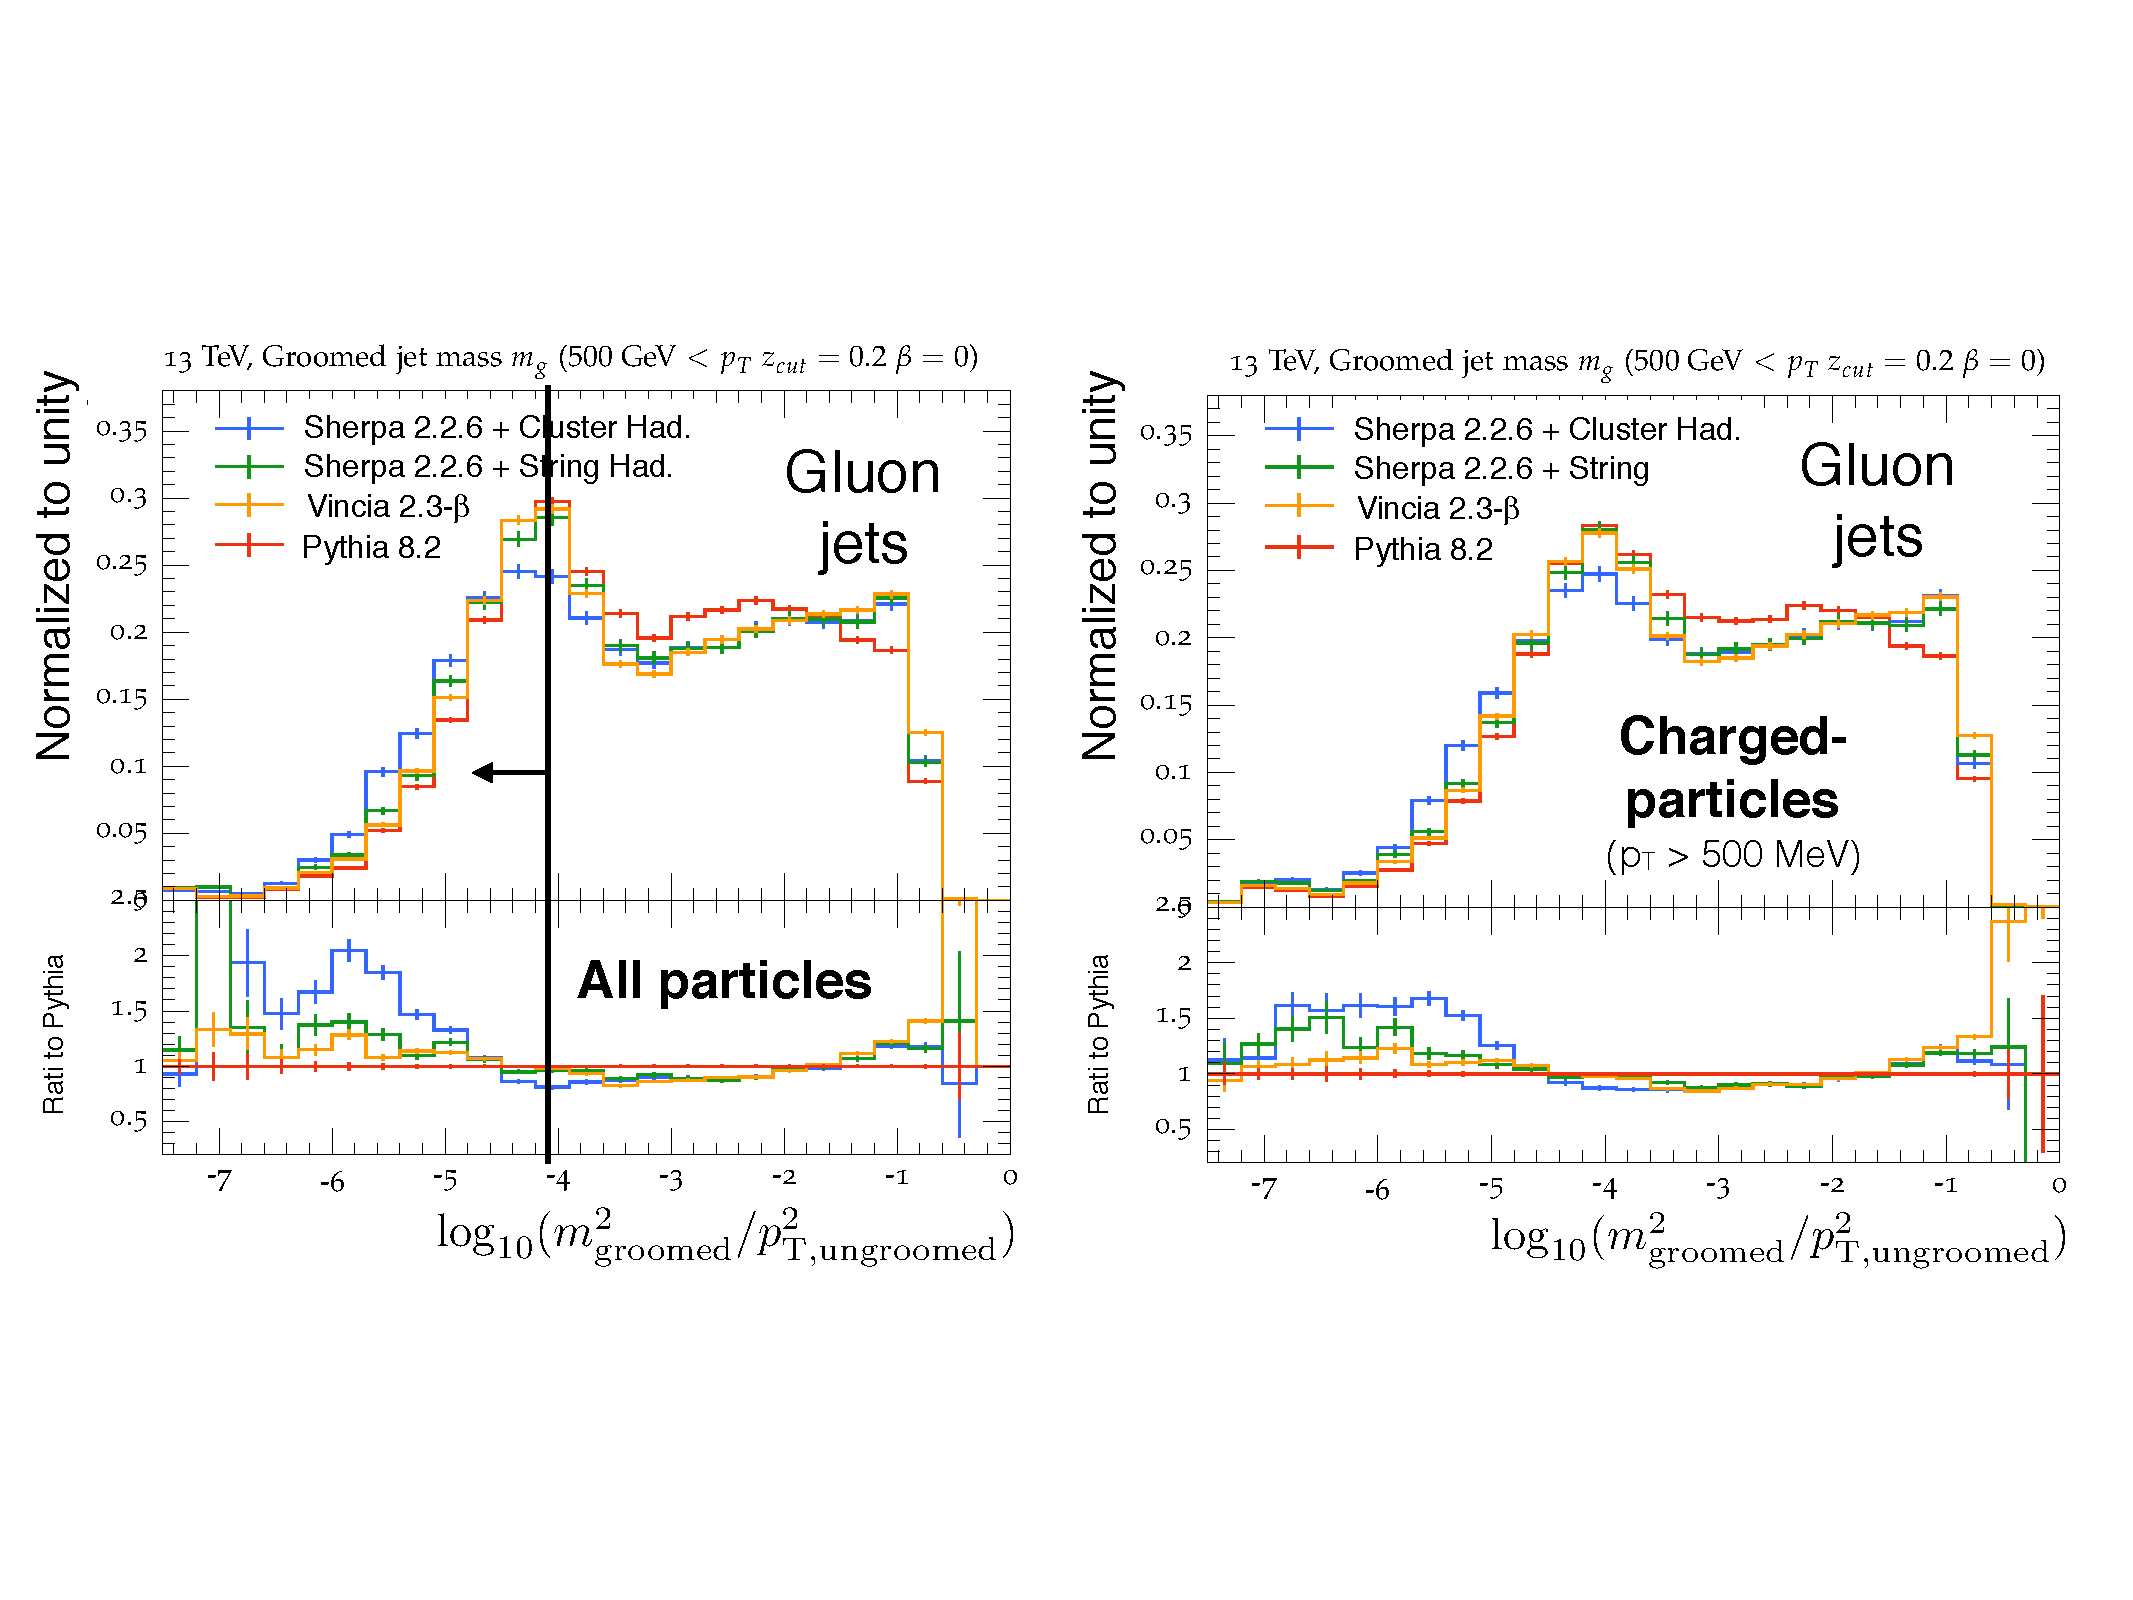
\includegraphics[width=0.95\textwidth]{figs/NPbumptracks.pdf}
\caption{The binned differential cross-section for the groomed jet mass using various Monte Carlo models and for all particle (left) and charged-particles only (right).  The vertical line with the arrow in the left plot shows the bin boundary for the lowest mass bin in the recent ATLAS measurements~\cite{Aaboud:2017qwh,Aad:2019vyi}.}
\label{fig:jets:np:tracks}
\end{figure}

The non-perturbative region is often avoided, but these studies indicate that there may be interesting and useful insight to learn from future studies that probe the differential cross section for the mass and potentially related observables.

\clearpage

\subsection{Monte Carlo tuning with jet substructure observables}
\label{sec:jets:mc}

While the jet mass differential cross section holds great potential for Monte Carlo tuning, it is only one of many.  The last several years have produced numerous measurements of jet and jet substructure observables at the LHC. 
Some of these measurements have been motivated by improving parton distribution functions and testing perturbative QCD predictions, 
while others have been designed to improve jet modeling by providing new and better inputs to Monte Carlo tuning.
Some of these, like the fragmentation functions~\cite{Aad:2019onw}, have been used for years to tune Monte Carlo predictions, 
while others, like the Lund Jet Plane~\cite{lundAtlas}, are measurements of observables which have only recently been proposed~\cite{lundPlane}.

With all of these observables, it is useful to consider which measurements are the most constraining for tuning jet modeling.
This is important for motivating future measurements, and can also be used to understand characteristics of the most effective observables.
This study compares several classes of variables in order to provide a more in-depth understanding of the interplay between observables and tuning.
Several simplifications were made in order to ease the comparisons. 
To remove any dependence on topologies, only measurements in dijet events are considered, and only 13 TeV measurements are used.
While both ATLAS and CMS have produced several measurements of jet substructure observables, only ATLAS measurements are considered, since there are more available measurements.
Currently, two measurements are considered: the soft drop mass measurement~\cite{Aaboud:2017qwh} and a measurement of a variety of jet substructure observables~\cite{Aaboud:2019aii}.


These studies scan a similar set of parameters as the ATLAS A14 tune~\cite{ATL-PHYS-PUB-2014-021}, focusing on parameters which are sensitive to parton showers and hadronization.
In addition to parameters which were considered for A14, one additional parameter, \texttt{StringPT:sigma}, is included due to its sensitivity to hadronization.
The list of parameters and their ranges of allowed values are shown in Table~\ref{tab:parameterSpace}.
The parameter space is scanned using a sampling of 300 different configurations determined by PROFESSOR2~\cite{Buckley:2009bj}, and the results are fit with a 3rd order polynomial.
%For the soft drop observables (SDO) results, each configuration is run with PYTHIA8~\cite{Sjostrand:2014zea} using a PhaseSpace:pTHatMin of 300 GeV, 
Each configuration is run with \texttt{PhaseSpace:pTHatMin} of 400 GeV, using 200,000 events per configuration. 
This allows sufficient sampling of the parameter space for the specific $p_{T}$ cuts of each analysis. 

\begin{table}[ht!]
\caption{Choices of parameters to tune, and their maximum and minimum values.}
\centering\begin{tabular}{ | c | | c | c | } \hline
                                     & Min. Value   & Max. Value    \\ \hline
\texttt{SigmaProcess:alphaSvalue}             &  0.12        & 0.15    \\ \hline
\texttt{BeamRemnants:primordialKThard}        &  1.5         & 2.0     \\ \hline
\texttt{SpaceShower:pT0Ref}                   &  0.75        & 2.0     \\ \hline
\texttt{SpaceShower:pTmaxFudge}               &  0.5         & 1.5     \\ \hline
\texttt{SpaceShower:pTdampFudge}              &  1.0         & 1.5     \\ \hline
\texttt{SpaceShower:alphaSvalue}              &  0.10        & 0.15    \\ \hline
\texttt{TimeShower:alphaSvalue}               &  0.10        & 0.15    \\ \hline
\texttt{StringPT:sigma}                       &  0.3         & 0.37    \\ \hline
\texttt{MultipartonInteractions:pT0Ref}       &  1.5         & 3.0     \\ \hline
\texttt{MultipartonInteractions:alphaSvalue}  &  0.1         & 0.15    \\ \hline
\end{tabular}
\label{tab:parameterSpace}
\end{table}

Several sets of tunes are compared in order to disentangle different effects from the measurement. 
Two sets of tunes are compared in order to disentangle the impact of different effects on the tuning.
In all cases, the results are compared for four different observables:
the soft drop jet mass distribution for $\beta=0$, the soft drop jet mass distribution for $\beta=2$, 
the number of subjets in a soft-dropped jet $N_{\mathrm{subjets}}$, and $\mathrm{ECF}_2^{\mathrm{norm}}$.
The two mass measurements provide insight into different aspects of the tune; $\beta=0$ is more sensitive to the perturbative parton shower information, 
while $\beta=2$ is more affected by hadronization. The number of subjets is sensitive to the hard splittings within a jet, and $\mathrm{ECF}_2^{\mathrm{norm}}$ is more sensitive to the 
distribution of energy within the jet. The event and jet selection is defined in the respective papers, and is taken from their RIVET routines~\cite{Buckley:2010ar}.

The first tune comparison studies the sensitivity to the $p_T$ selection and binning used for the measurements. Two different tunes are performed, each using only the jet mass as input.
The first tune uses the three jet mass measurements with different soft drop parameters from Ref.~\cite{Aaboud:2017qwh}, using the inclusive $p_T$ binning. 
The second uses the $p_T$-binned measurements from the same measurement. 
The results of these three tunes are shown in Figure~\ref{massOnlyTune}. 
The two tunes which use the high-$p_T$ measurement produce similar tunes, with similar uncertainties on their parameters. 
While the $p_T$-binned result in principle provides more access to information such as quark-gluon differences or scaling with $p_T$, the impact on the results is small. 


\begin{figure}
\begin{center}
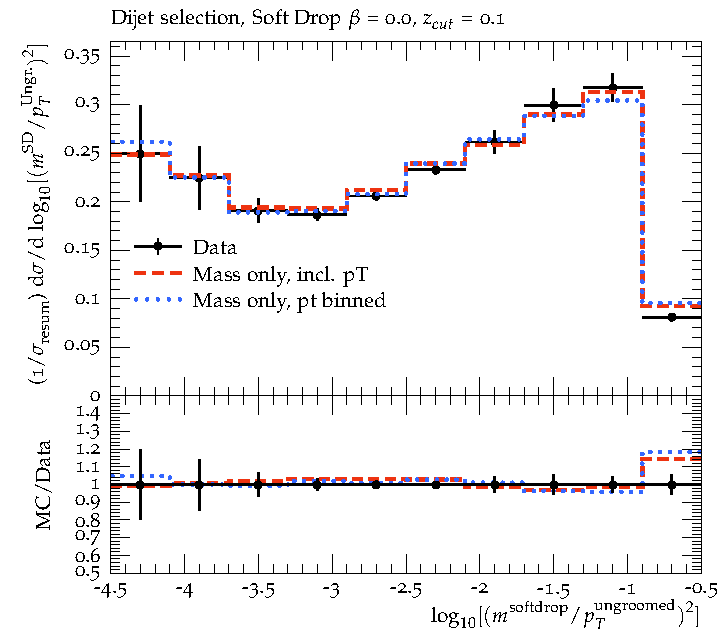
\includegraphics[width=0.49\textwidth]{figs/RivetPlotsMassOnly/SoftDropMass/d01-x01-y01.pdf} \hfill
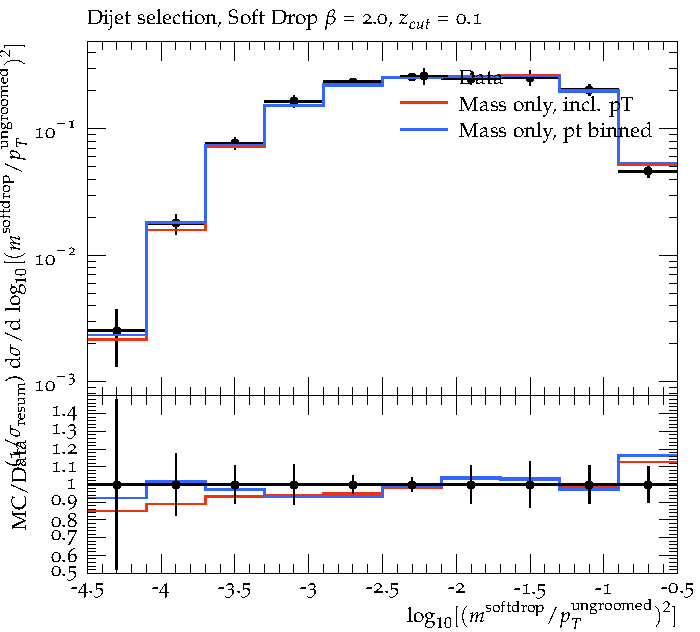
\includegraphics[width=0.49\textwidth]{figs/RivetPlotsMassOnly/SoftDropMass/d03-x01-y01.pdf} \hfill
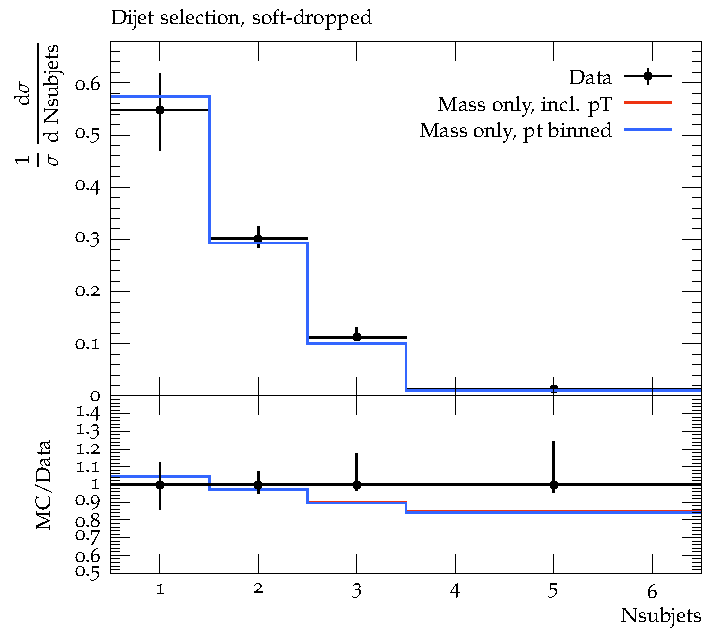
\includegraphics[width=0.49\textwidth]{figs/RivetPlotsMassOnly/ATLAS_2019_I1724098/d23-x01-y01.pdf} \hfill
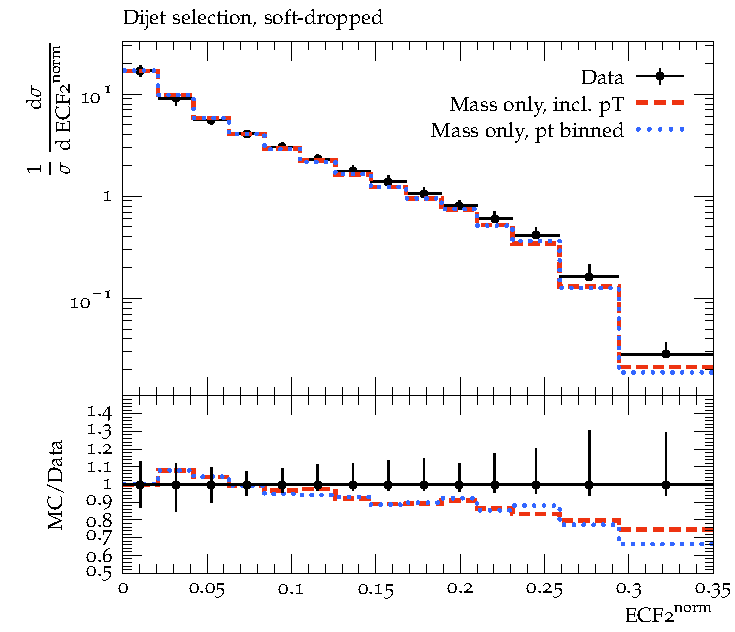
\includegraphics[width=0.49\textwidth]{figs/RivetPlotsMassOnly/ATLAS_2019_I1724098/d27-x01-y01.pdf} \hfill
\end{center}
\label{massOnlyTune}
\end{figure}


The second set of tunes compares the results from each individual measurement. The first of these is the same tune as before, using the $p_T$ inclusive soft drop jet mass measurements.
The second tune uses the measurements of six jet substructure measurements in jets groomed with the soft drop algorithms, as measured in Ref~\cite{Aaboud:2019aii}.
These measurements are compared to two standard tunes: the ATLAS A14 tune and the MONASH tune.~\footnote{The ATLAS tune is slightly different than the standard ATLAS tune, since it uses the ATLAS tune results, but does not use the recommended PDF set.}
The results of these are shown in Figure~\ref{allTune}. 
In general, the agreement of substructure observables is improved by the use of substructure measurements compared to the ATLAS A14 tune or the MONASH tune.
As demonstrated in the mass distribution, the tunes from this study seem to lack some information about the fixed-order tune, 
and so they likely need to be combined with other measurements for full accuracy. 


\begin{figure}
\begin{center}
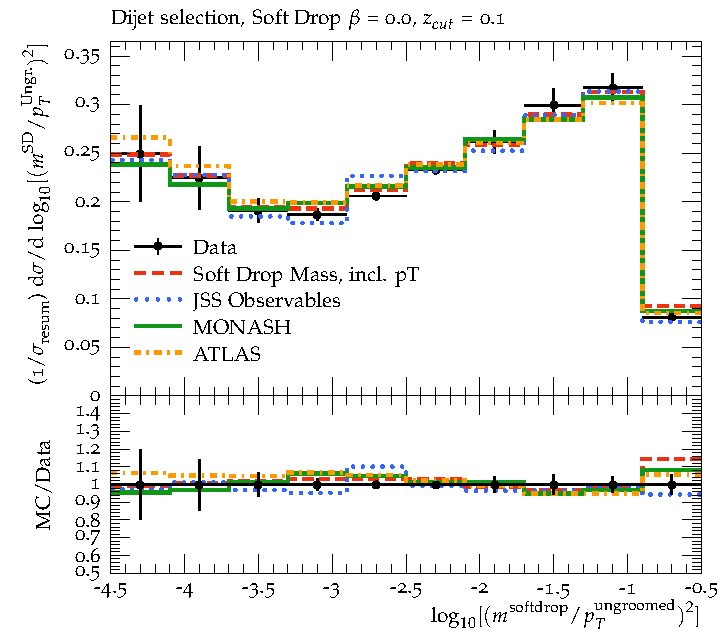
\includegraphics[width=0.49\textwidth]{figs/RivetPlotsFinal/SoftDropMass/d01-x01-y01.pdf} \hfill
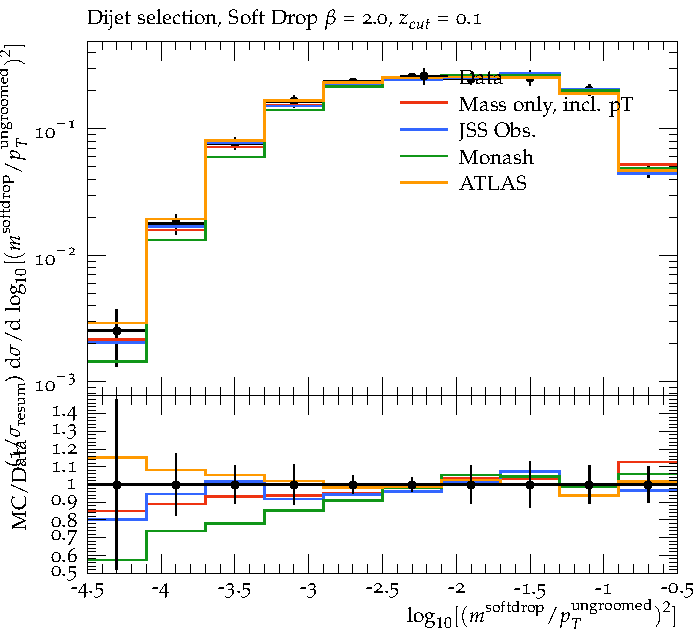
\includegraphics[width=0.49\textwidth]{figs/RivetPlotsFinal/SoftDropMass/d03-x01-y01.pdf} \hfill
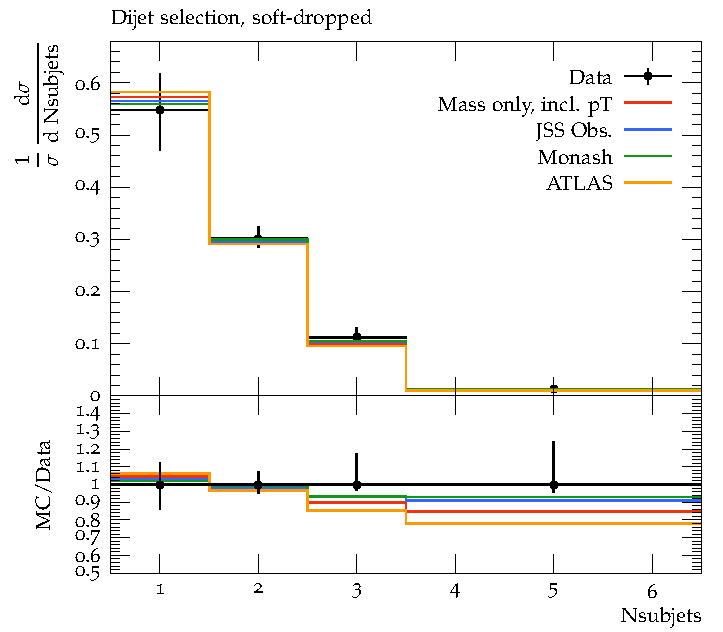
\includegraphics[width=0.49\textwidth]{figs/RivetPlotsFinal/ATLAS_2019_I1724098/d23-x01-y01.pdf} \hfill
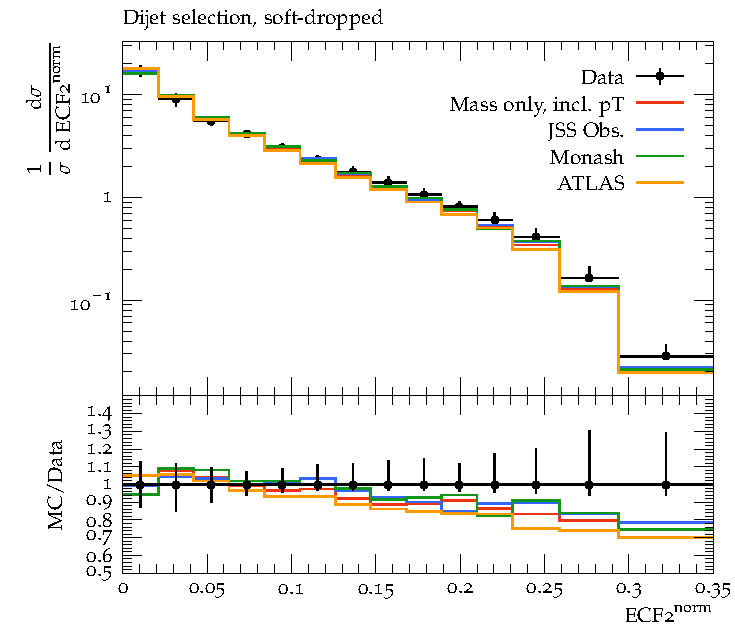
\includegraphics[width=0.49\textwidth]{figs/RivetPlotsFinal/ATLAS_2019_I1724098/d27-x01-y01.pdf} \hfill
\end{center}
\label{allTune}
\end{figure}


The full set of tuned parameters and their uncertainties is shown in Table~\ref{tab:tuneResults}. 


%\clearpage
%\begin{landscape}
\begin{table}[ht!]
\resizebox{\textwidth}{!}{

\centering\begin{tabular}{ | c | | c | c | c | c | c |} \hline
                                     & MONASH   & ATLAS  & SDM Incl Pt   & SDM Pt Binned & JSS Observables  \\ \hline
\texttt{SigmaProcess:alphaSvalue}             &  0.130   & 0.144  & 0.126+/-0.003 & 0.126+/-0.001 & 0.133+/-0.002 \\ \hline
\texttt{BeamRemnants:primordialKThard}        &  1.8     & 1.72   & 1.825+/-0.055 & 1.794+/-0.011 & 1.785+/-0.048 \\ \hline
\texttt{SpaceShower:pT0Ref}                   &  2.0     & 1.30   & 1.668+/-0.100 & 1.744+/-0.078 & 1.721+/-0.121 \\ \hline
\texttt{SpaceShower:pTmaxFudge}               &          & 0.95   & 1.150+/-0.054 & 1.071+/-0.014 & 1.036+/-0.034 \\ \hline
\texttt{SpaceShower:pTdampFudge}              &          & 1.21   & 1.214+/-0.058 & 1.157+/-0.011 & 1.284+/-0.040 \\ \hline
\texttt{SpaceShower:alphaSvalue}              &  0.1365  & 0.125  & 0.123+/-0.003 & 0.126+/-0.001 & 0.130+/-0.003 \\ \hline
\texttt{TimeShower:alphaSvalue}               &  0.1365  & 0.126  & 0.132+/-0.001 & 0.131+/-0.001 & 0.133+/-0.000 \\ \hline
\texttt{StringPT:sigma}                       &  0.335   &        & 0.348+/-0.003 & 0.350+/-0.003 & 0.333+/-0.006 \\ \hline
\texttt{MultipartonInteractions:pT0Ref}       &  2.28    & 1.98   & 2.000+/-0.100 & 2.181+/-0.049 & 2.441+/-0.148 \\ \hline
\texttt{MultipartonInteractions:alphaSvalue}  &  0.130   & 0118   & 0.116+/-0.003 & 0.126+/-0.002 & 0.128+/-0.003 \\ \hline
\end{tabular}}
\caption{Values of tuned parameters.}
\label{tab:tuneResults}
\end{table}
%\end{landscape}
%\clearpage



More study is needed in order to fully understand the implications of these results, but there are a few interesting comments. 
The soft drop jet mass distribution was designed to study perturbative QCD, but also had several bins sensitive to non-perturbative effects. 
With these preliminary studies, it appears to be as effective in tuning as Ref~\cite{Aaboud:2019aii}, even though it uses fewer observables. 
This is likely due to the factorization of different effects in the soft drop mass distribution, allowing it to be simultaneously sensitive to fixed order effects, the parton shower, and hadronization. 
This shows that factorization is important, and that it is important to be sensitive to a variety of effects when creating these tunes.








\subsection{Probing higher-order effects in PSMC}
\label{sec:jets:psmc}

\subsubsection{Triple Collinear Splitting Functions}


Dire~\cite{Hoche:2015sya}.  PFN~\cite{Komiske:2018cqr}.

Here, we will discuss now useless triple-collinear corrections to Dire were, and
how awesome double-soft contributions are.

\dots some Dire bullet points
\begin{itemize}
\item parton showers serve two purposes: $1)$ the distribution of low-multiplicity
(hard-scattering) states over states of arbitrarily high multiplicity, as well
as $2)$ generating the effect of resummation for observable depending only on 
low-multiplicity configurations.
\item these two purposes are often in conflict, e.g.\ choices to improve
$2)$ often limit the potential to improve $1)$ -- and vice versa. these
conflicts are not apparent at lowest (i.e.\ leading) order.
\item parton showers typically include states distributed with leading-order 
(leading-logarithmic) rate in their emission- and no-emission probabilities.
\item the rate of subsequent splittings is independent of the rate of
previous splittings, and the evolution scales at which splittings occur is
successively ordered -- such that resummation can occur.
\item with demand for more precise event generation, improved parton showers
are necessary. For example, the use of NLO PDFs (as e.g.\ mandated in NLO+PS
matching) in the parton shower in principle requires parton showers beyond
lowest order.
\item one way to improve the all-order behavior of the parton shower (point $2)$ 
above) while preserving a systematically improvable state distribution (point $1)$ 
above) is to consistently include higher-order and higher-multiplicity 
splitting functions in the parton shower.
\item several such configurations are shown in 
Figure~\ref{fig:jets:np:triplecollineardiagrams}. Such configurations are
already approximated through the iterated application of leading-order
splittings, albeit with incorrect rate (e.g.\ if the polarisation of 
the intermediate gluon in 
Figs.~\ref{fig:jets:np:triplecollineardiagrams1}-\ref{fig:jets:np:triplecollineardiagrams4},
\ref{fig:jets:np:triplecollineardiagrams7}-\ref{fig:jets:np:triplecollineardiagrams8}
is omitted, leading to an incorrect modulation of azimuthal angles,
or simply disregarding the interference between
$C_F$-type and $C_A$-type color structures from 
Figs.~\ref{fig:jets:np:triplecollineardiagrams7}-\ref{fig:jets:np:triplecollineardiagrams8})
or in a phase-space constrained by successive ordering (easily leading to the 
incorrect phase space volume, and thus failing to recover known anomalous
dimensions)
\item the correct final result is obtained by including the 
configurations~\ref{fig:jets:np:triplecollineardiagrams}
as new rates to the parton shower, and subtracting from these new rates
the leading-order result. This subtraction will, given a suitable definition
of the leading-order shower, act to ensure local finiteness of the new, 
subtracted, rates. We will call these subtracted rates ``corrections".
\item In~\cite{Hoche:2017iem}, triple-collinear corrections from diagram
similar to~\ref{fig:jets:np:triplecollineardiagrams2} were considered, with
the difference that instead of the primary parton (indicated with a double 
line), one of the quarks in the loop was considered as ``hard". Such
configurations give, upon integration, give rise to the flavor-changing 
DGLAP kernels $P_{qq'}$ and $P_{q\bar q}$. We
will call this ``triple-collinear" correction.
\item \cite{Dulat:2018vuy} considered all the 
diagrams~\ref{fig:jets:np:triplecollineardiagrams}
in the soft limit, and included all necessary virtual corrections obtained
by moving the cuts in the indiviual diagrams in all possible ways. We
will call this ``double-soft" correction.
\item It should be noted that there is overlap between the
triple-collinear and double-soft limits. A complete differential calculation 
that consistently (i.e.\ without overlap) includes all components has yet
to be produced. Thus, we assess the potential to find observables
that discriminate between leading-order and next-to-leading order
results separately for triple-collinear and double-soft corrections.
\item We find that the effect triple-collinear corrections (which integrate to
the DGLAP kernels $P_{qq'}$ and $P_{q\bar q}$) is difficult to pinpoint. 
It is somewhat surprising that the impact is almost vanishing.
\item We find that double-soft corrections have sizable impact, and can
easily be filtered out of the data. This is expected, since the theoretical
description of soft gluons changes significantly.
\item \emph{more to come, going to sleep now\dots}
\end{itemize}

\begin{figure}[h!]
\subfigure[blub]{
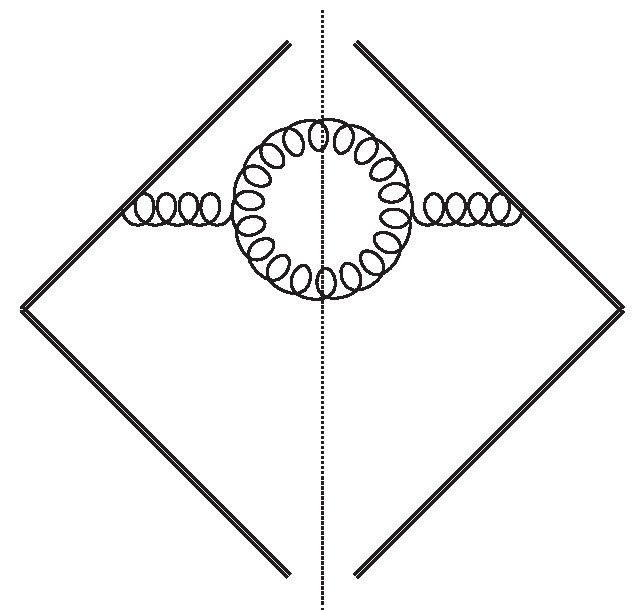
\includegraphics[width=0.23\textwidth]{figs/nlo_real_vpcg.pdf}
\label{fig:jets:np:triplecollineardiagrams1}
}
\subfigure[blub]{
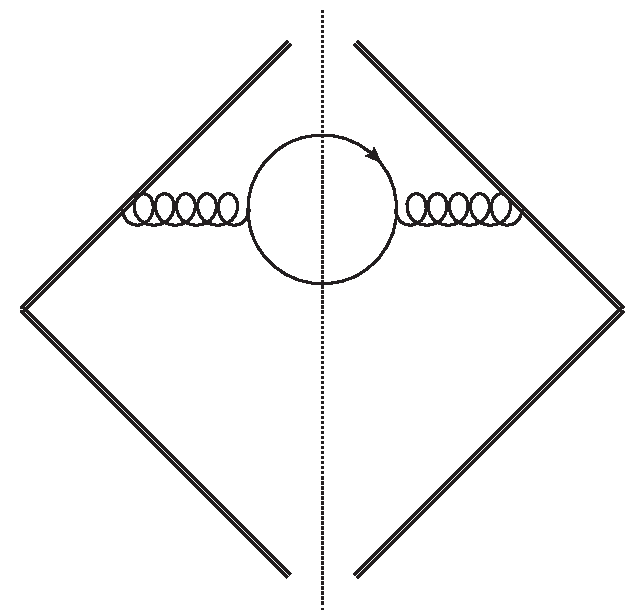
\includegraphics[width=0.23\textwidth]{figs/nlo_real_vpcq.pdf}
\label{fig:jets:np:triplecollineardiagrams2}
}
\subfigure[blub]{
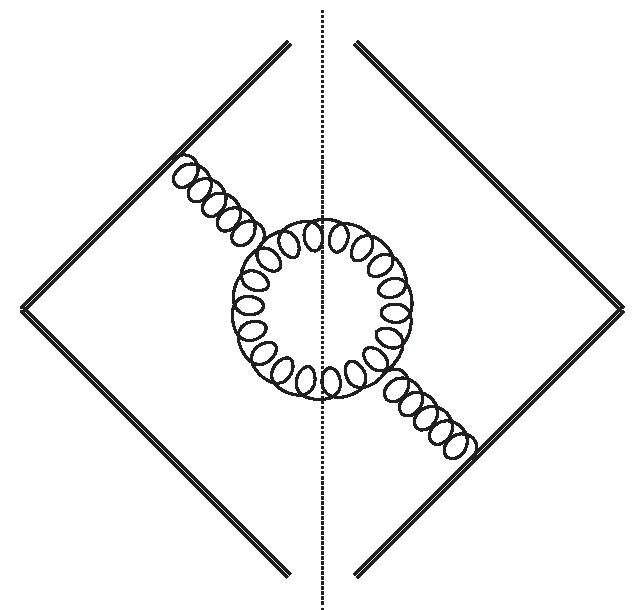
\includegraphics[width=0.23\textwidth]{figs/nlo_real_vpsg.pdf}
\label{fig:jets:np:triplecollineardiagrams3}
}
\subfigure[blub]{
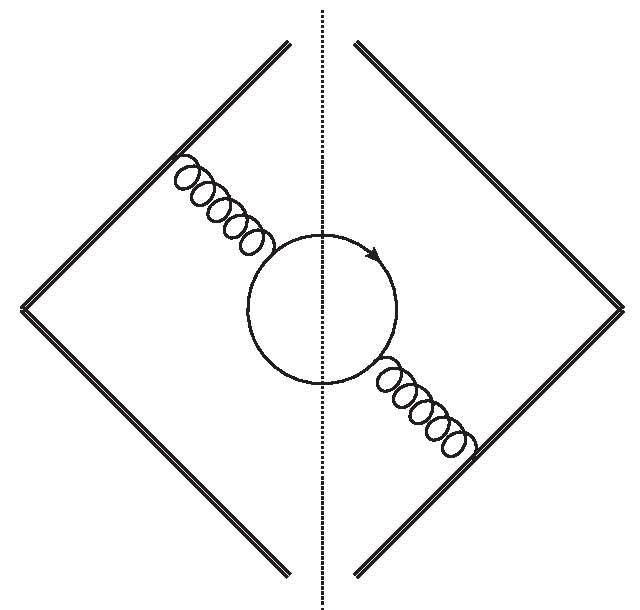
\includegraphics[width=0.23\textwidth]{figs/nlo_real_vpsq.pdf}
\label{fig:jets:np:triplecollineardiagrams4}
}
\\
\subfigure[blub]{
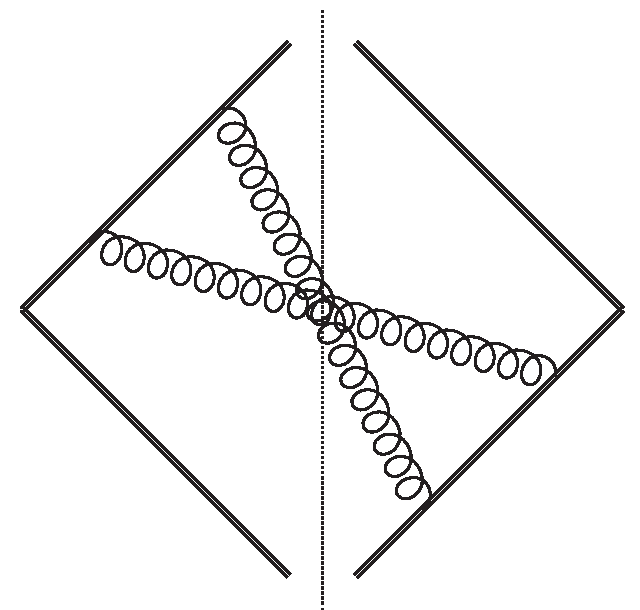
\includegraphics[width=0.23\textwidth]{figs/nlo_real_box1.pdf}
\label{fig:jets:np:triplecollineardiagrams5}
}
\subfigure[blub]{
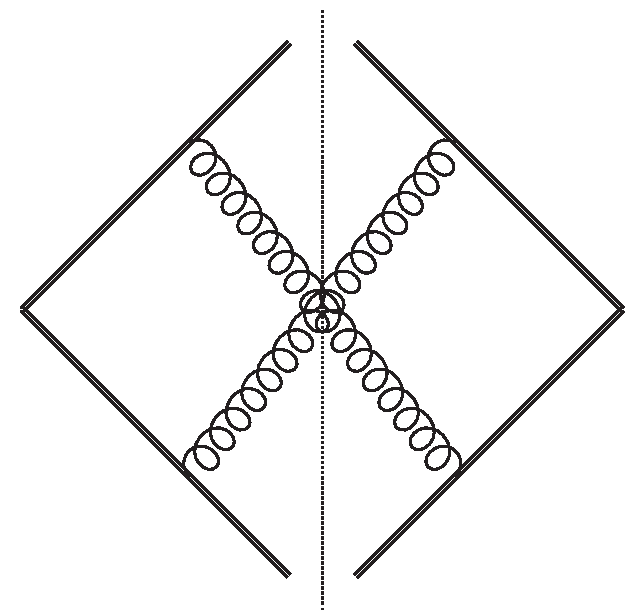
\includegraphics[width=0.23\textwidth]{figs/nlo_real_box2.pdf}
\label{fig:jets:np:triplecollineardiagrams6}
}
\subfigure[blub]{
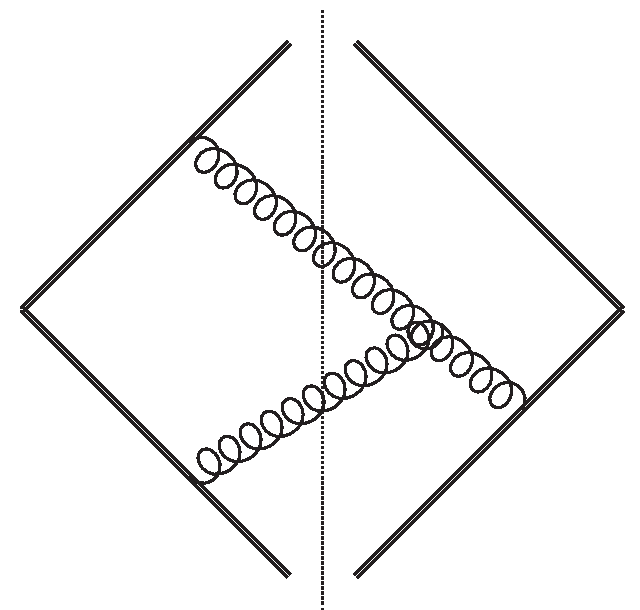
\includegraphics[width=0.23\textwidth]{figs/nlo_real_tgc1.pdf}
\label{fig:jets:np:triplecollineardiagrams7}
}
\subfigure[blub]{
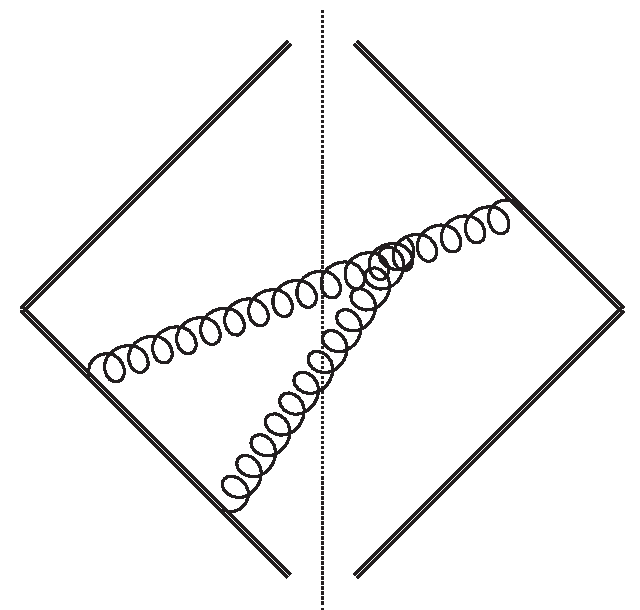
\includegraphics[width=0.23\textwidth]{figs/nlo_real_tgc2.pdf}
\label{fig:jets:np:triplecollineardiagrams8}
}
\caption{Replace me with proper diagrams!}
\label{fig:jets:np:triplecollineardiagrams}
\end{figure}

\begin{figure}[h!]
\centering
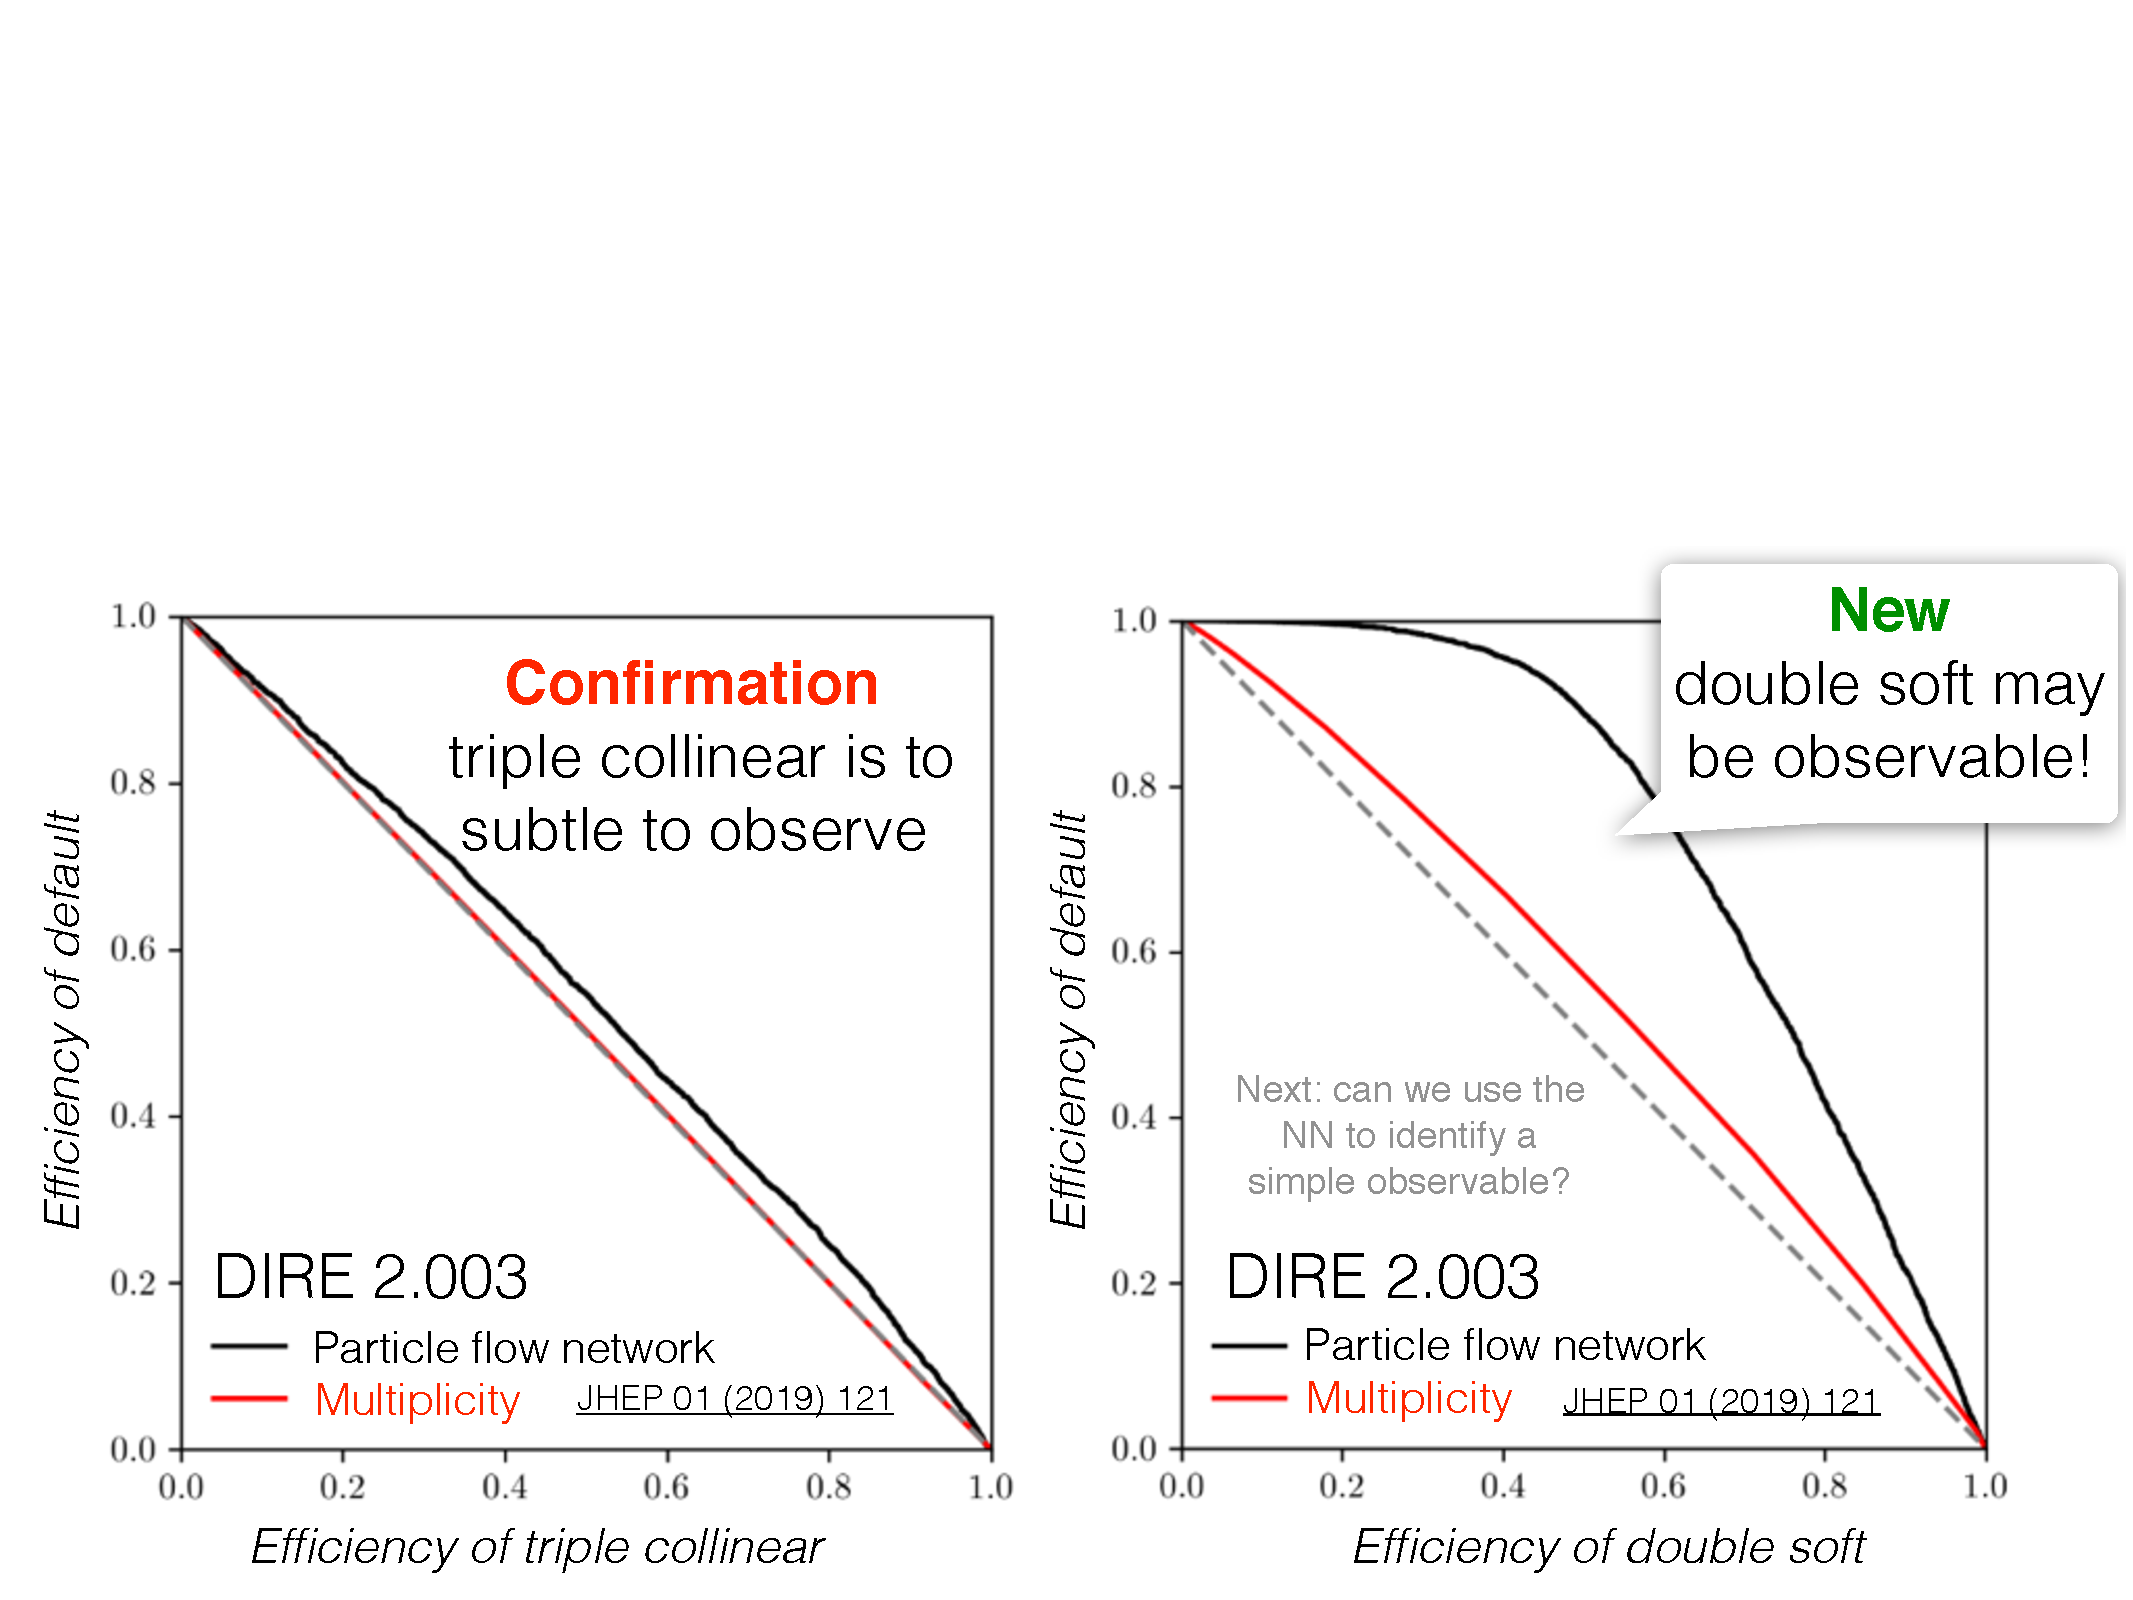
\includegraphics[width=0.85\textwidth]{figs/triplecollinear.pdf}
\caption{Replace me with proper plots!}
\label{fig:jets:np:triplecollinearNN}
\end{figure}






\clearpage

\subsection{q/g tagging in VBF and VBS}
\label{sec:jets:vbsbvf}

Describe Fig.~\ref{fig:jets:qg}.

\begin{figure}[h!]
\centering
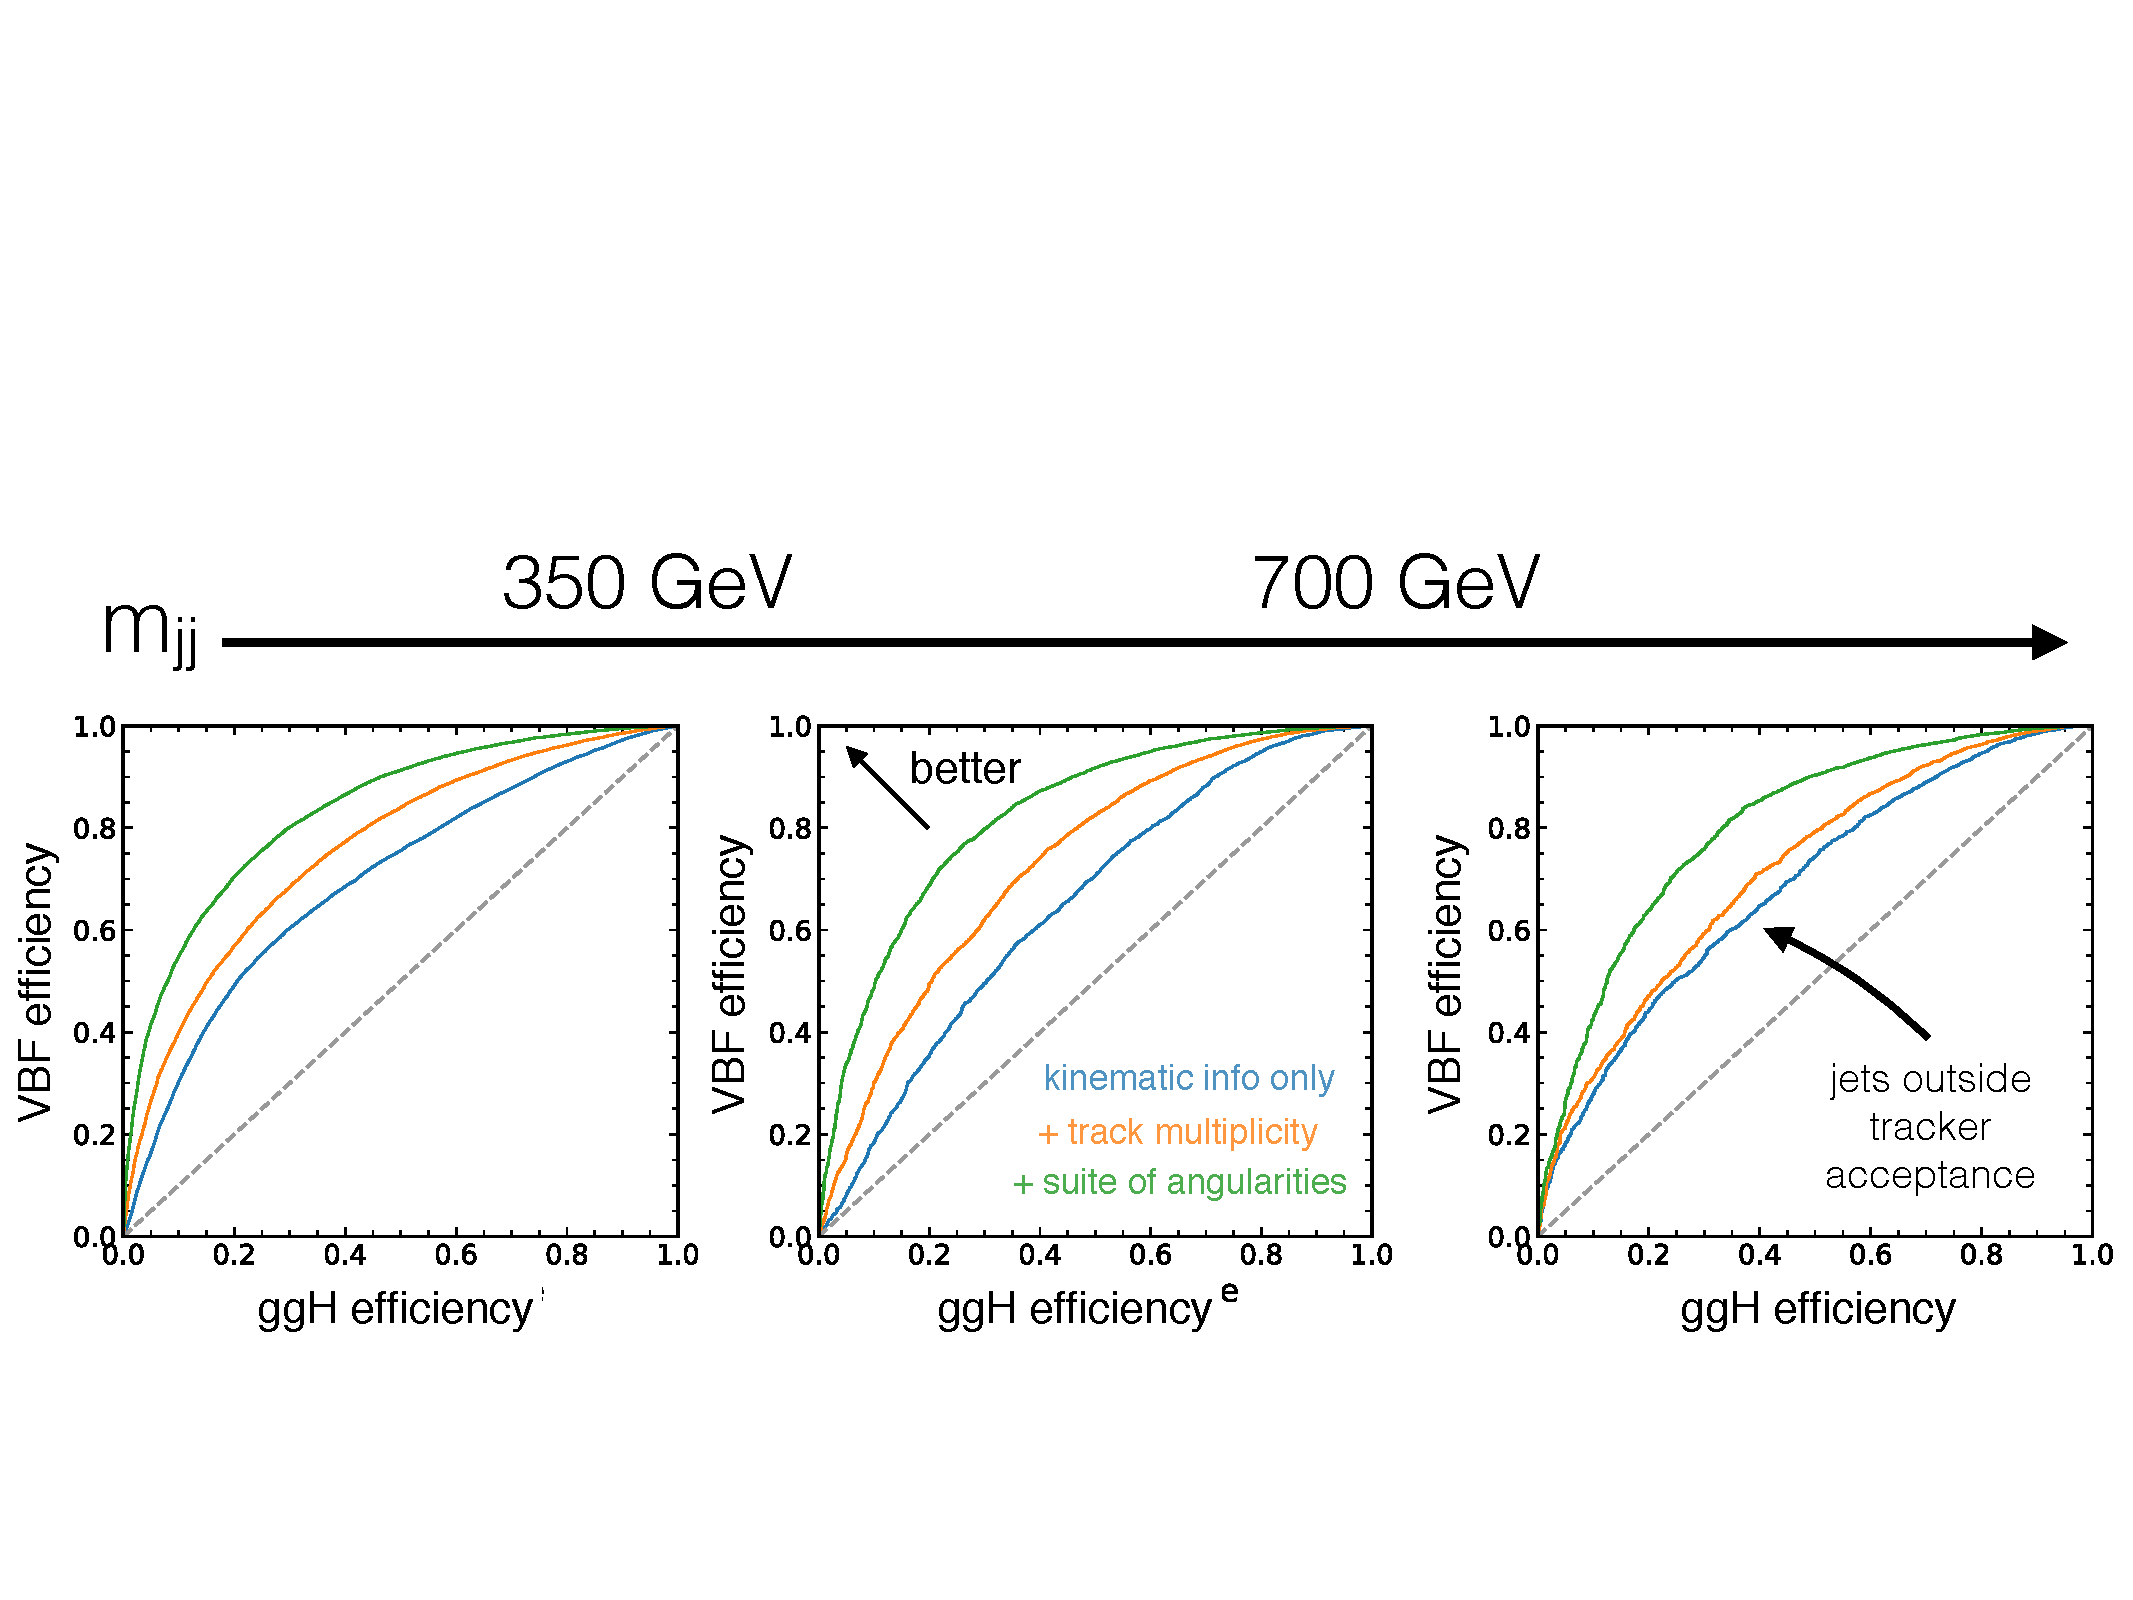
\includegraphics[width=0.95\textwidth]{figs/qgstudy.pdf}
\caption{blah}
\label{fig:jets:qg}
\end{figure}

\subsection{\textsc{Squirrel} for the Gluon PDF}
\label{sec:jets:pdf}

\subsection{The gluon PDF (a.k.a Suppressing the QUark in the Region of RElative Large-$x$)}
(Simone, Gregory, Eric)

Parton Distribution Functions (PDFs) describe the non-perturbative dynamics of quarks and gluons in the protons that take part in high-energy collisions. Therefore, they are a key ingredient for every theoretical prediction that aims to describe particle interactions at high-energy colliders such as the LHC. As a consequence, their precise determination is of utmost importance for LHC phenomenology. 
%
The non-perturbative nature of PDFs hampers their determination from first principles.
%
However, for inclusive enough processes, they are universal, i.e.\, up to power corrections, they do not depend on the particular process, and they can be determined by fitting data from previous experiments. Moreover, although they are themselves non-perturbative objects, their dependence on the energy is governed by the DGLAP equation and the evolution kernels can be computed as a power expansion in the strong coupling. This implies that data collected at past experiments, at different energies, can be used to constrain PDFs. 

Traditionally, the main source of uncertainties assigned to the determination of PDFs arises from the experimental error of the data that enter the fit.~\footnote{Very recently, the inclusion of theory uncertainties in PDF determination has also been achieved~\cite{Harland-Lang:2018bxd,AbdulKhalek:2019ihb,AbdulKhalek:2019bux}} In extreme regions of phase-space, for instance at small- or large-$x$, the experimental uncertainties typically deteriorate and one has to face a reduced number of data points. This is reflected in PDFs which are largely unconstrained in these regions. 
%
For instance, the large PDF uncertainty in the $x\to 1$ region has a negative impact on searches for new and heavy states.
%
 Although this will probably not wash out a potential discovery, it will definitely obscure the nature and the properties of the new state, such as its mass and its couplings. 
%
The way to reduce this PDF uncertainty is to include in the fit data at larger $x$. This cause interesting theoretical issues, because fixed-order perturbation theory becomes less reliable and one should supplement theoretical predictions with threshold resummation, as studied for instance in~\cite{Corcella:2005us,Sato:2013wea,Westmark:2013vea,Bonvini:2015ira,Accardi:2014qda}.


In this study, we focus on the gluon PDF in the region of relatively large longitudinal momentum fraction, $x\sim 10^{-1}$ \sm{check}. The datasets that mostly constrain the gluon in this region are the inclusive jet spectra, in the region of the jet transverse momentum above 1~TeV and the production of top quark pairs. From a theoretical point of view, both processes are known to very high accuracy, i.e. next-to-next-to-leading order (NNLO)~\cite{}. Phenomenologically, the two processes have pros and cons. Inclusive jet production features high statistics across a wide kinematical range and, consequently, even in the high $p_t$ region we are interested the experimental uncertainties do not exceed 10\%. However, because we are measuring inclusive jets we cannot distinguish the flavour content and the cross section is dominated by quark-quark scattering, which bear little information about the gluon PDF. 
%
On the other hand, at LHC energies, top pair production is dominated by gluon fusion and therefore offers a direct probe of the gluon luminosity. In this case, however, we pay a much higher price in terms of experimental uncertainties, essentially because we run out of statistics of values of the top transverse momentum much smaller than for inclusive jets. 
%
Ideally, we would like to exploit the vast jet samples collected by the LHC experiments to tease out more information about the gluon PDF. We immediately realise that one way of achieving this scope would be to supplement the inclusive jet $p_t$ spectrum with some information about the jet flavour. That is, we are going to explore the possibility of using the \emph{inclusive gluon-jet $p_t$} spectrum to extract parton densities, rather than its flavour-blind version.  Properly defining quark jets versus gluon jets is a very active area of jet substructure~\cite{} and indeed it was one of the focus of a past edition of the Les Houches proceedings~\cite{Badger:2016bpw} (see also the follow-up study~\cite{Gras:2017jty}). 


\begin{figure}
\begin{center}
\includegraphics[width=0.49\textwidth, page=9]{figs/fractions.pdf} \hfill
\includegraphics[width=0.49\textwidth, page=10]{figs/fractions.pdf}
\caption{Born-level studies of the flavour composition of dijet events at $\sqrt{s}=13$~TeV, as a function of the jet transverse momentum. The plot on the left shows the fractions of quark-initiated and gluon-initiated processes that contribute to a $gg$ final state. The plot of the right instead shows the fractional composition of the final state for any initial state.}
\label{fig:born_studies} 
\end{center}
\end{figure}

Before discussing how we can sensibly attach a flavour tag to a jet, let us perform a zeroth order test of this idea. Let us assume that we can indeed tag a gluon jet in the final state, the obvious question we should ask ourselves is how strongly the flavour of the final state, which we measure, is correlated with the flavour of the initial state, which intimately related to the parton densities we want to study. 
%
We can easily assess this correlation at Born level by explicitly consider $2 \to 2$ parton scattering and focussing on the two gluon ($gg$) final state. The left-hand plot of Fig.~\ref{fig:born_studies} shows the fraction of the $gg$ final state that originates from quark-anti-quark initial state ($q \bar q \to gg$) in red and the one from gluon-gluon initial state ($gg \to gg$)  in blue, as a function of the final-state transverse momentum for proton-proton collisions at $\sqrt{s}=13$~TeV (the plot uses the NLO PDF set CT14~\cite{Dulat:2015mca}). 
%
The result of this very first study is rather encouraging: in the region $p_t=1,2$~TeV we are interested, there is indeed very strong correlation between the initial- and final-state flavours. This is, of course, only a Born-level study and we can reasonably expect this correlation to deteriorate at higher-orders mostly due to large-angle radiation. 
%
Although a quantitative estimate of these effects goes beyond the scope of these proceedings, we do not expect them to be dramatic. In any case, one could in principle reduce such contributions with jet grooming. 
%
With the same Born-level setup, we can study how the different partonic final states contribute to the inclusive cross section. This is shown on the right-hand plot of Fig.~\ref{fig:born_studies}. As $p_t$ increases, the fraction of final-state quark rapidly increases. Indeed, the region of interest the $gg$ final state represents less than 10\% of the inclusive sample. This makes the enterprise of enhancing the $gg$ contributions (or, equivalently, suppressing the quarks) particularly challenging. 



\begin{figure}
\begin{center}
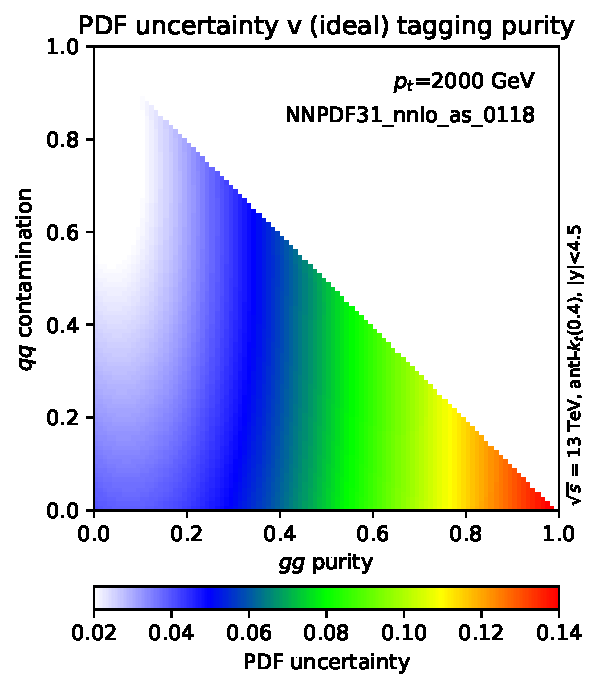
\includegraphics[width=0.42\textwidth, page=1]{figs/performance-plots.pdf} \hfill
\includegraphics[width=0.49\textwidth, page=2]{figs/performance-plots.pdf}
\caption{}
\label{fig:pdf_unc_studies} 
\end{center}
\end{figure}

The next step in our study is to evaluate the current PDF uncertainties, as a function of the final-state flavour composition. 
%
In order to do so, we imagine as a fist step to have at our disposal an idealised tagging procedure that allows us to freely enhance or depress the different partonic components of the final state. We will come back to actual realisations of this tagger later. 
%
In this context, we find useful to define the gluon-gluon ($gg$) purity as
\begin{equation}
gg \, \text{purity}= \frac{\sigma_{gg}}{\sigma_{qq}+\sigma_{qg}+\sigma_{gg}},
\end{equation}
where $\sigma_{ij}$ is the cross section for producing parton $i$ and $j$, evaluated at Born level.  In an analogous way, we can also define the $q q$ contamination is defined analogously, while $q g$ is then fixed by unitarity. Then, for given values $gg$ purity and $qq$ contamination we can evaluate the PDF uncertainty on the cross section.
%
 We decide to perform this estimate using the NNLO PDF set from NNPDF3.1~\cite{Ball:2017nwa} for jets at $2$~TeV.
 %
%The results are shown in Fig.~\ref{fig:pdf_unc_studies}, on the left. 
%
We actually already know from Fig.~\ref{fig:born_studies}, that in the inclusive, i.e.\ untagged, case correspond to $gg$ purity of the order 5\% at $p_t=2$~TeV, while $qq$ and $qg$ makes up roughly 55\% and 40\% of the inclusive sample, respectively. 
%
From the left-hand plot on Fig.~\ref{fig:pdf_unc_studies}, we can then read-off the PDF uncertainty to be of the order of a few percent. This is reflects the fact that the quark parton densities are fairly-well constrained in the region of interest. 
As we move to higher values of the $gg$ purity, the less constrained gluon PDFs start to play a more significant role and, as a consequence, the overall uncertainties goes up. For instance, if we were able to devise a tagger that purifies the $gg$ final state to 80\%, we would increase the PDF uncertainty from 2\% to 12\%. 


\begin{figure}
\begin{center}
\includegraphics[width=0.49\textwidth, page=4]{figs/performance-plots.pdf} \hfill
\includegraphics[width=0.49\textwidth, page=5]{figs/performance-plots.pdf}
\caption{}
\label{fig:performance_studies} 
\end{center}
\end{figure}


\subsection{The highest energy gluons at the LHC}
\label{sec:jets:highest}

In addition to their use for precision QCD, high $p_T$ gluons may also be a powerful tool for BSM searches.  In particular, Fig.~\ref{fig:born_studies} showed that the fraction of gluon-gluon final states decreases rapidly near the kinematic limit.  Suppose that there is a new particle at high invariant mass which decays to gluons.  Such particles are present in many BSM models, including a significant fraction of those that were proposed to explain the early Run 2 diphoton excess~\cite{Khachatryan:2016hje,Aaboud:2016tru}.  While the jets from this signal would be gluons, the dominant background at high $m_{jj}$ is from quark jets.  Therefore, a powerful gluon tagger may be able to significantly improve the sensitivity of a search to these di-gluon resonances\footnote{During the preparation of these proceedings, this was also pointed out by Ref.~\cite{Nayak:2019quy}.}.  In fact, the theoretical efficacy of gluon tagging improves the higher the mass of the new resonance: the background becomes more quark-like and quark and gluon jets become more different due to their increasing constituent multiplicity.  These theoretical gains are limited by experimental challenges related to the reconstruction of high energy constituents inside the dense core of high $p_T$ jets.  For a typical working point of 50\% gluon jet efficiency and a quark jet rejection of 10, the in-principle gain in significance to high-mass gluon resonances is $0.5^2/\sqrt{0.1^2}=2.5$.

\subsection{Conclusion and Outlook}
\label{sec:jets:conclusion}
The jet subgroup at Les Houches 2019 concentrated their effort on the study of gluonic jets across four decades of energy, which are explored by the LHC. 
%
In the low-energy regime jets are sensitive to the non-perturbative dynamics of QCD and their description is beyond the jurisdiction of the standard first-principle approach based on perturbative field theory. Therefore, phenomenological models are usually employed to describe the non-perturbative parton-to-hadron transition. 
%
In our study, we have first addressed some of qualitative features of the groomed jet mass distribution in the non-perturbative regime and then turned our attention to the possibility of employing jet substructure variables to test and, eventually, improve on, the modelling of non-perturbative corrections in Monte Carlo event generators. 

As we go up in energy, we enter the regime where we expect parton-shower algorithms to correctly capture the relevant physics. In this context, we have investigated the impact of higher-order corrections to the splitting kernels that are at the core of any parton-branching algorithm. In particular, we have exploited modern machine-learning techniques in order to design observables that are sensitive to triple-collinear and double-soft corrections. 
%
At high energy, the issue of determining whether a given jet can be labelled as quark-initiated or gluon-initiated becomes central in Higgs physics and in the context of searches for particles and interactions beyond the Standard Model. Therefore, we have studied the performance of quark/gluon tagging in vector-boson-fusion and vector-boson-scattering analyses. Inspired by quark/gluon tagging in searches, we have explored the possibility of measuring gluon-jet transverse momentum distributions as a probe of parton distribution functions at high, i.e.\ 1~TeV, scale.
%
Finally, we have discussed how to probe the most energetic gluons at the LHC.


This report testifies that the jet subgroup have enjoyed a fruitful workshop, characterised by lively discussions and cross-pollination of ideas not only between theory and experimental communities but also between different methodologies, such as first-principle calculations in field theory, Monte Carlo simulations and machine-learning techniques. 
%
We are confident that these results, in some cases still preliminary, are already seeding new ideas and research projects which we look forward to further developing at the next edition of this workshop. 	



\subsection*{Acknowledgments}

We thank the participants of Les Houches 2019 for a lively environment and useful discussions.
%%
BN is supported in part by the Office of High Energy Physics of the U.S. Department of Energy under Contract No. DE-AC02-05CH11231.
%
SM is also supported by the curiosity-driven grant ``Using jets to challenge the Standard Model of particle physics" from Universit\`a di Genova.

\bibliography{lh2019}

\end{document}
